% ===== Appendix =====
\section{Appendix}\label{appendix}

% ----- A. Per-domain accuracy and the excluded sports domain -----
\subsection{A. Per-category and per-domain accuracy and the excluded
sports domain}\label{a.-per-domain-accuracy-and-the-excluded-sports-domain}

Table \ref{tbl:bycategory} gives the full per-category judge-label
breakdown behind Section 5.1. Mean log-probability also stratifies: the
model is \emph{least} confident on the obscure pre-cutoff items
(refusals, concentrated post-cutoff, are themselves fluent and
high-confidence; Section 5.3).

\begin{table}[!htbp]
\small
\centering
\caption{Judge-label counts, accuracy, and mean per-token log-probability by
category.\label{tbl:bycategory}}
\begin{tabular}{@{}lrrrrrr@{}}
\toprule
category & n & correct & refusal & wrong & accuracy & mean logprob \\\midrule
well-known (pre-cutoff) & 143 & 89 & 0 & 54 & 62.2\% & \(-0.120\) \\
obscure (pre-cutoff) & 153 & 51 & 0 & 102 & 33.3\% & \(-0.149\) \\
post-cutoff & 488 & 95 & 147 & 246 & 19.5\% & \(-0.145\) \\
\midrule
\textbf{total} & 784 & 235 & 147 & 402 & 30.0\% & \(-0.141\) \\
\bottomrule
\end{tabular}
\end{table}

\begin{table}[!htbp]
\small
\centering
\caption{ConfabQA cell counts: 4 domains \(\times\) 3 categories,
\(n = 784\).\label{tbl:cells}}
\begin{tabular}{@{}lrrrr@{}}
\toprule
domain & well-known & obscure & post-cutoff & total \\\midrule
science & 42 & 45 & 119 & 206 \\
history & 33 & 37 & 127 & 197 \\
culture & 34 & 34 & 121 & 189 \\
cinema & 34 & 37 & 121 & 192 \\
\textbf{total} & \textbf{143} & \textbf{153} & \textbf{488} &
\textbf{784} \\
\bottomrule
\end{tabular}
\end{table}

\begin{table}[!htbp]
\small
\centering
\caption{Per-domain accuracy, overall and by cutoff
class.\label{tbl:appdomain}}
\begin{tabular}{@{}lrrrll@{}}
\toprule
domain & n & correct & accuracy & pre-cutoff & post-cutoff \\\midrule
science & 206 & 75 & 36.4\% & 25/87 (28.7\%) & 50/119 (42.0\%) \\
history & 197 & 67 & 34.0\% & 54/70 (77.1\%) & 13/127 (10.2\%) \\
culture & 189 & 65 & 34.4\% & 42/68 (61.8\%) & 23/121 (19.0\%) \\
cinema & 192 & 28 & 14.6\% & 19/71 (26.8\%) & 9/121 (7.4\%) \\
\bottomrule
\end{tabular}
\end{table}

History remains the strongest pre-cutoff domain (77.1\%); cinema the
weakest overall (14.6\%). Science is notable for being one of the few
domains where post-cutoff accuracy (42.0\%, 50/119) is \emph{higher}
than pre-cutoff (28.7\%), driven by a handful of post-cutoff items about
Anthropic, OpenAI, and SpaceX that the model has apparently learned via
post-training data.

\subsubsection{A.1 The excluded sports
domain}\label{a.1-the-excluded-sports-domain}

An earlier iteration of the benchmark included a fifth domain,
\textbf{sports}, with the same three-category design applied to MLB
World Series, NFL Super Bowl, and Grand Slam tennis questions. On a
26-item run of Qwen3-1.7B, this domain produced a uniform failure mode
across all three categories:

\begin{table}[!htbp]
\small
\centering
\caption{The excluded sports domain: accuracy by category on the 26-item
run.\label{tbl:sports}}
\begin{tabular}{@{}lrrrr@{}}
\toprule
domain & well\_known & obscure & post\_cutoff & overall \\\midrule
sports & 0/10 (0.0\%) & 0/10 (0.0\%) & 0/6 (0.0\%) & 0/26 (0.0\%) \\
\bottomrule
\end{tabular}
\end{table}

Judge labels: 23 \texttt{wrong}, 3 \texttt{refusal}, 0 \texttt{correct}.
Examples of confidently wrong responses:

\begin{center}
\small
\begin{tabular}{@{}
  >{\raggedright\arraybackslash}p{(\linewidth - 6\tabcolsep) * \real{0.2500}}
  >{\raggedright\arraybackslash}p{(\linewidth - 6\tabcolsep) * \real{0.2500}}
  >{\raggedright\arraybackslash}p{(\linewidth - 6\tabcolsep) * \real{0.2500}}
  >{\raggedleft\arraybackslash}p{(\linewidth - 6\tabcolsep) * \real{0.2500}}@{}}
\toprule
\begin{minipage}[b]{\linewidth}\raggedright
question
\end{minipage} & \begin{minipage}[b]{\linewidth}\raggedright
gold
\end{minipage} & \begin{minipage}[b]{\linewidth}\raggedright
model said
\end{minipage} & \begin{minipage}[b]{\linewidth}\raggedleft
\(\bar\ell\)
\end{minipage} \\\midrule
Men's 2023 French Open winner & Novak Djokovic & ``Alexander Zverev
defeated Djokovic in the final'' & \(-0.087\) \\
2023 World Series winner & Texas Rangers & ``Los Angeles Dodgers
defeated Chicago Cubs in seven games'' & \(-0.091\) \\
2009 World Series winner & New York Yankees & ``St.~Louis Cardinals
defeated the New York Yankees'' & \(-0.094\) \\
\bottomrule
\end{tabular}
\end{center}

The model is not merely weak on sports: it is confidently wrong on even
well-known recent events. Dropping sports from the main 4-domain
analysis is motivated rather than convenient: the \emph{zero-correct}
well-known cell means the within-pre-cutoff probe on this domain alone
would have zero positive examples, making the disconfound test
undefined. The source files (\texttt{data/sources/sports/*.json}) remain
in the repository and the question-set generator can re-include the
domain by reverting one line of \texttt{01\_question\_set.py:DOMAINS}.
The 26-item sports archive is at
\texttt{data/responses\_v1\_133/spo\_*.json}.

\subsubsection{A.2 Text-level confidence
figure}\label{a.2-text-level-confidence-figure}

Figure \ref{fig:confidence} shows the Section 5.2 text-level confidence
distributions. Panel (b) shows that the correctness/cutoff interaction
is also visible in joint logprob-entropy space, with post-cutoff items
concentrated in the lower-confidence region of the plane (lower mean
logprob, higher mean entropy) and pre-cutoff correct items concentrated
near zero. The substantial overlap between pre-cutoff-correct and
post-cutoff-correct in the high-confidence corner is the visual analogue
of ``logprob alone does not separate confabulation from correct''.

\begin{figure}
\centering
\pandocbounded{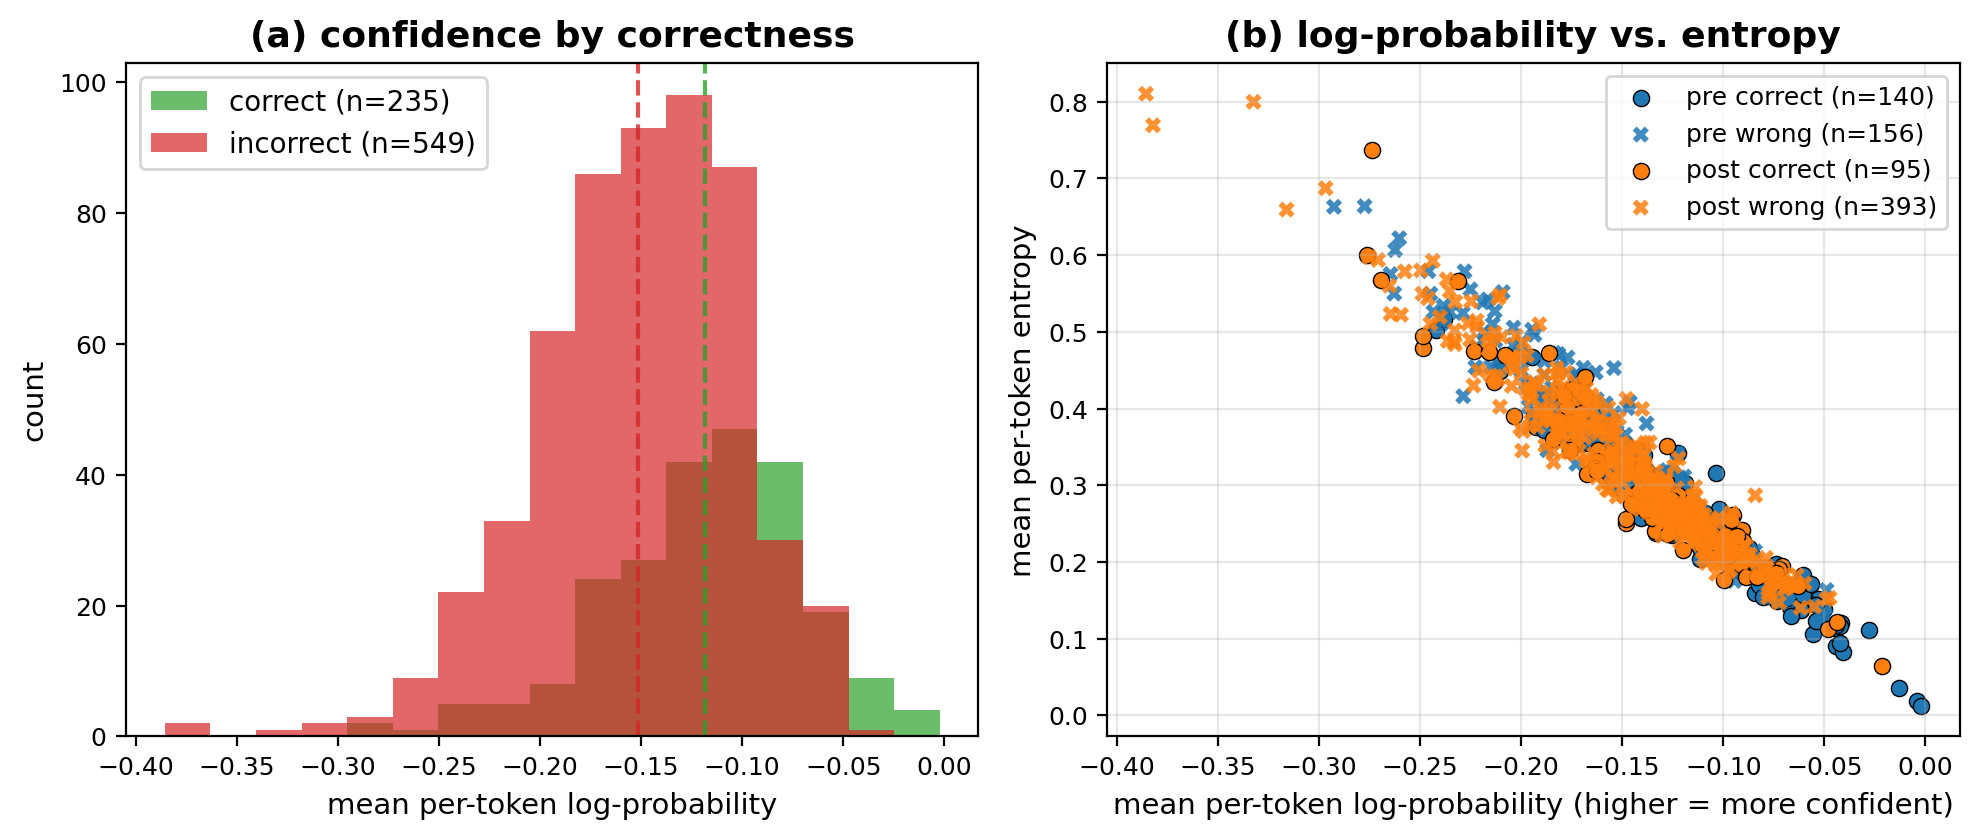
\includegraphics[keepaspectratio,alt={Text-level confidence. (a) Histogram
  of per-item mean per-token log-probability under greedy decoding, split by judge
  correctness label: the two distributions overlap substantially, their means differing by
  \textbackslash approx 0.05 nats. (b) Per-item mean log-probability vs.~mean entropy,
  colored by cutoff class, marker by correctness. Pre/post-cutoff items occupy
  distinguishable regions but with heavy overlap, especially among confident
  wrongs.}]{figures/qwen3_1_7b/confidence_merged.png}}
\caption{Text-level confidence. \textbf{(a)} Histogram of per-item mean
per-token log-probability under greedy decoding, split by judge
correctness label: the two distributions overlap substantially, their
means differing by \(\approx 0.05\) nats. \textbf{(b)} Per-item mean
log-probability vs.~mean entropy, colored by cutoff class, marker by
correctness. Pre/post-cutoff items occupy distinguishable regions but
with heavy overlap, especially among confident
wrongs.}\label{fig:confidence}
\end{figure}

\subsubsection{A.3 Highest-confidence confabulations and
refusals}\label{a.3-highest-confidence-confabulations-and-refusals}

Table \ref{tbl:topwrong} lists the Section 5.3 case studies; they
exemplify the canonical failure mode, a plausible-sounding specific
answer with a recognizable name from the right time period and category,
at high text-level confidence. Four of the five confabulations are
obscure pre-cutoff items, where the model had partial training-data
exposure to the gold answer; the fifth is post-cutoff, where it had
none.

\begin{table}[!t]
\small
\caption{The five highest-confidence confabulations (top block) and refusals
(bottom block; all post-cutoff). Questions and answers are excerpts from the
released response files.\label{tbl:topwrong}}
\begin{tabular}{@{}
  >{\raggedright\arraybackslash}p{(\linewidth - 8\tabcolsep) * \real{0.1412}}
  >{\raggedright\arraybackslash}p{(\linewidth - 8\tabcolsep) * \real{0.2941}}
  >{\raggedright\arraybackslash}p{(\linewidth - 8\tabcolsep) * \real{0.1647}}
  >{\raggedright\arraybackslash}p{(\linewidth - 8\tabcolsep) * \real{0.3412}}
  >{\raggedleft\arraybackslash}p{(\linewidth - 8\tabcolsep) * \real{0.0588}}@{}}
\toprule
id & question (abridged) & gold & model said (excerpt) & $\bar\ell$ \\
\midrule
\textbf{\emph{wrong}} & & & & \\
cin\_pc\_41 & Ridley Scott's November 2024 sequel to \emph{Gladiator}? &
Gladiator II & ``There is no film directed by Ridley Scott that is a
sequel to \emph{Gladiator}\ldots{}'' & $-0.047$ \\
cul\_ob\_12 & Which 1971 Walker Percy novel won the National Book Award?
& Love in the Ruins & ``\ldots was `The Crying of Lot 49'\,'' & $-0.049$ \\
cin\_ob\_24 & Who directed `Three Colors: Blue' (1993)? & Krzysztof
Kieslowski & ``\ldots was directed by Jean-Pierre Jeunet'' & $-0.049$ \\
his\_ob\_35 & Who was the 27th US President, 1909--1913? & William
Howard Taft & ``\ldots was Theodore Roosevelt'' & $-0.050$ \\
his\_ob\_30 & Who was Chancellor of West Germany, 1969--1974? & Willy
Brandt & ``\ldots was Konrad Adenauer'' & $-0.052$ \\
\textbf{\emph{refusal}} & & & & \\
his\_pc\_38 & Treasury Secretary in the second Trump administration,
January 2025? & Scott Bessent & ``As of January 2025, there is no
Secretary of the Treasury\ldots{}'' & $-0.049$ \\
cin\_pc\_14 & Who starred in Bong Joon-ho's 2025 film `Mickey 17'? &
Robert Pattinson & ``As of my knowledge cutoff in 2023, there is no 2025
film titled \emph{Mickey 17}\ldots{}'' & $-0.055$ \\
cul\_pc\_20 & Which Taylor Swift album was released on April 19, 2024? &
The Tortured Poets Department & ``As of my knowledge cutoff in 2024,
there is no official announcement\ldots{}'' & $-0.060$ \\
cin\_pc\_114 & 2025 Best Supporting Actor Academy Award, for `A Real
Pain'? & Kieran Culkin & ``As of the 2025 Academy Awards, there is no
official announcement\ldots{}'' & $-0.064$ \\
his\_pc\_33 & US Attorney General in the second Trump administration,
February 2025? & Pam Bondi & ``As of February 2025, there is no United
States Attorney General\ldots{}'' & $-0.067$ \\
\bottomrule
\end{tabular}
\end{table}

\subsubsection{A.4 Hidden-state geometry
figures}\label{a.4-unsupervised-hidden-state-geometry}

\begin{figure}
\centering
\pandocbounded{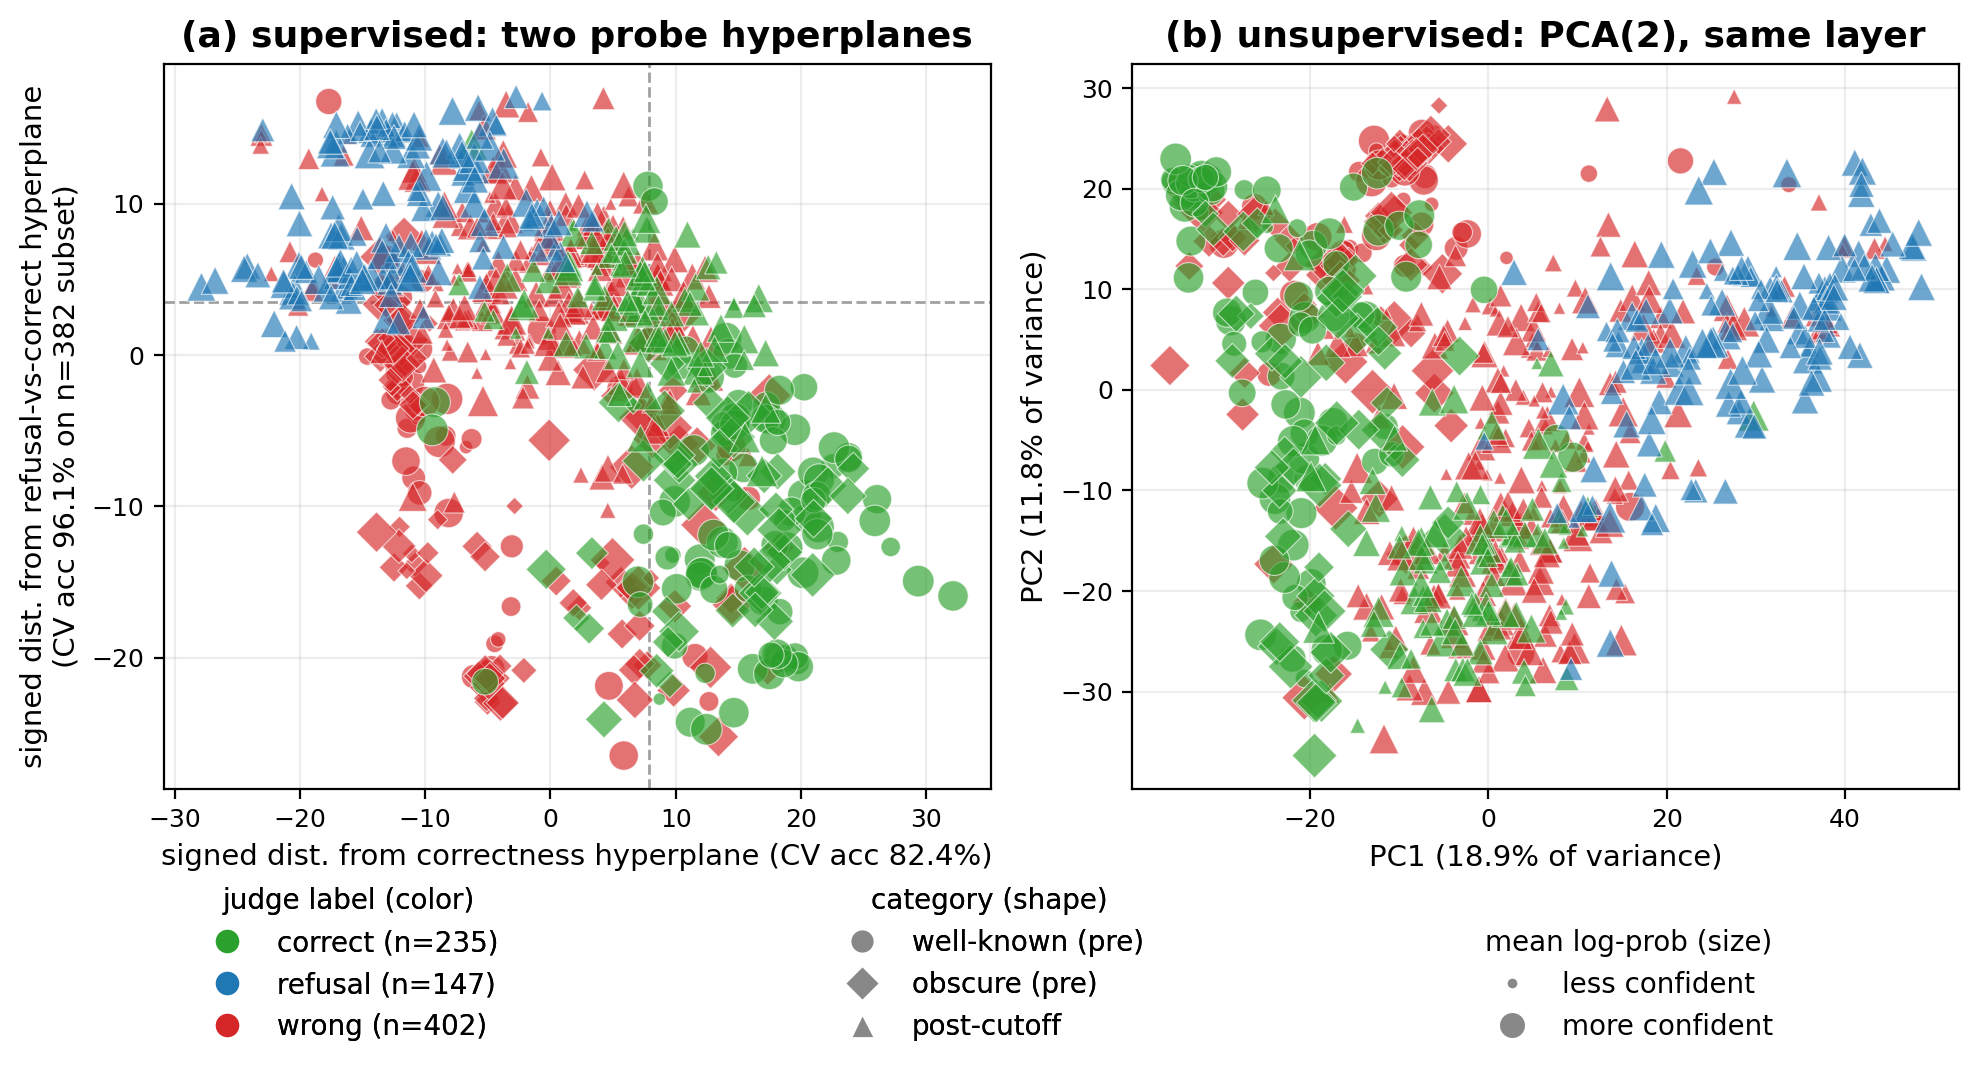
\includegraphics[keepaspectratio,alt={Confabulation Atlas (layer 18 hidden
  state). Each point is one question: color = judge label (green correct, blue refusal,
  red wrong), shape = category (circle well-known, diamond obscure, triangle post-cutoff),
  size = mean per-token log-probability (larger = more confident). (a) Supervised
  projection. X: signed distance to the correctness hyperplane (target judge\_label ==
  "correct", all n=784, 5-fold CV acc 82.4\textbackslash\%). Y: signed distance to the
  refusal-vs-correct hyperplane (target refusal vs correct, fit on the n=382
  refusal+correct subset, 5-fold CV acc 96.1\textbackslash\%, orthogonalized against X for
  plotting; raw angle between the two hyperplane normals in 16-d PCA space is
  55.7\^{}\textbackslash circ). Wrong items, never seen during the Y fit, fall between the
  refusal pole (top) and the correct pole (bottom). (b) Unsupervised control. PCA(2) of
  the same hidden state, same encoding: even without supervision, PC1 and PC2 already
  carry visible refusal-vs-rest structure (a probe on PC1+PC2 alone reaches
  86.9\textbackslash\% on the refusal-vs-wrong target, vs.~73.2\textbackslash\% majority).
  The ``atlas'' is therefore not an artifact of supervised projection: the underlying
  hidden state already separates refusal in its top-variance directions. Whether the
  correctness separation visible in panel (a) reflects model-internal self-knowledge or
  simply prompt-readable features is the subject of Section
  5.6.}]{figures/qwen3_1_7b/atlas_merged_layer18.png}}
\caption{\textbf{Confabulation Atlas (layer 18 hidden state; Section
5).} Each point is one question: color = judge label (green correct,
blue refusal, red wrong), shape = category (circle well-known, diamond
obscure, triangle post-cutoff), size = mean per-token log-probability.
\textbf{(a) Supervised projection.} \textbf{X:} signed distance to the
correctness hyperplane (all \(n=784\), 5-fold CV acc \(82.4\%\)).
\textbf{Y:} signed distance to the refusal-vs-correct hyperplane (fit on
the \(n=382\) refusal+correct subset, CV acc \(96.1\%\), orthogonalized
against X for plotting; raw angle between the normals in 16-d PCA space
\(55.7^\circ\)). Wrong items, never seen during the Y fit, fall between
the refusal pole (top) and the correct pole (bottom).
\textbf{(b) Unsupervised control.} PCA(2) of the same states: even
without supervision, PC1 and PC2 already carry visible refusal-vs-rest
structure. Whether the \emph{correctness} separation in (a) reflects
self-knowledge or prompt-readable features is the subject of Section
5.6.}\label{fig:atlas}
\end{figure}

\begin{figure}
\centering
\pandocbounded{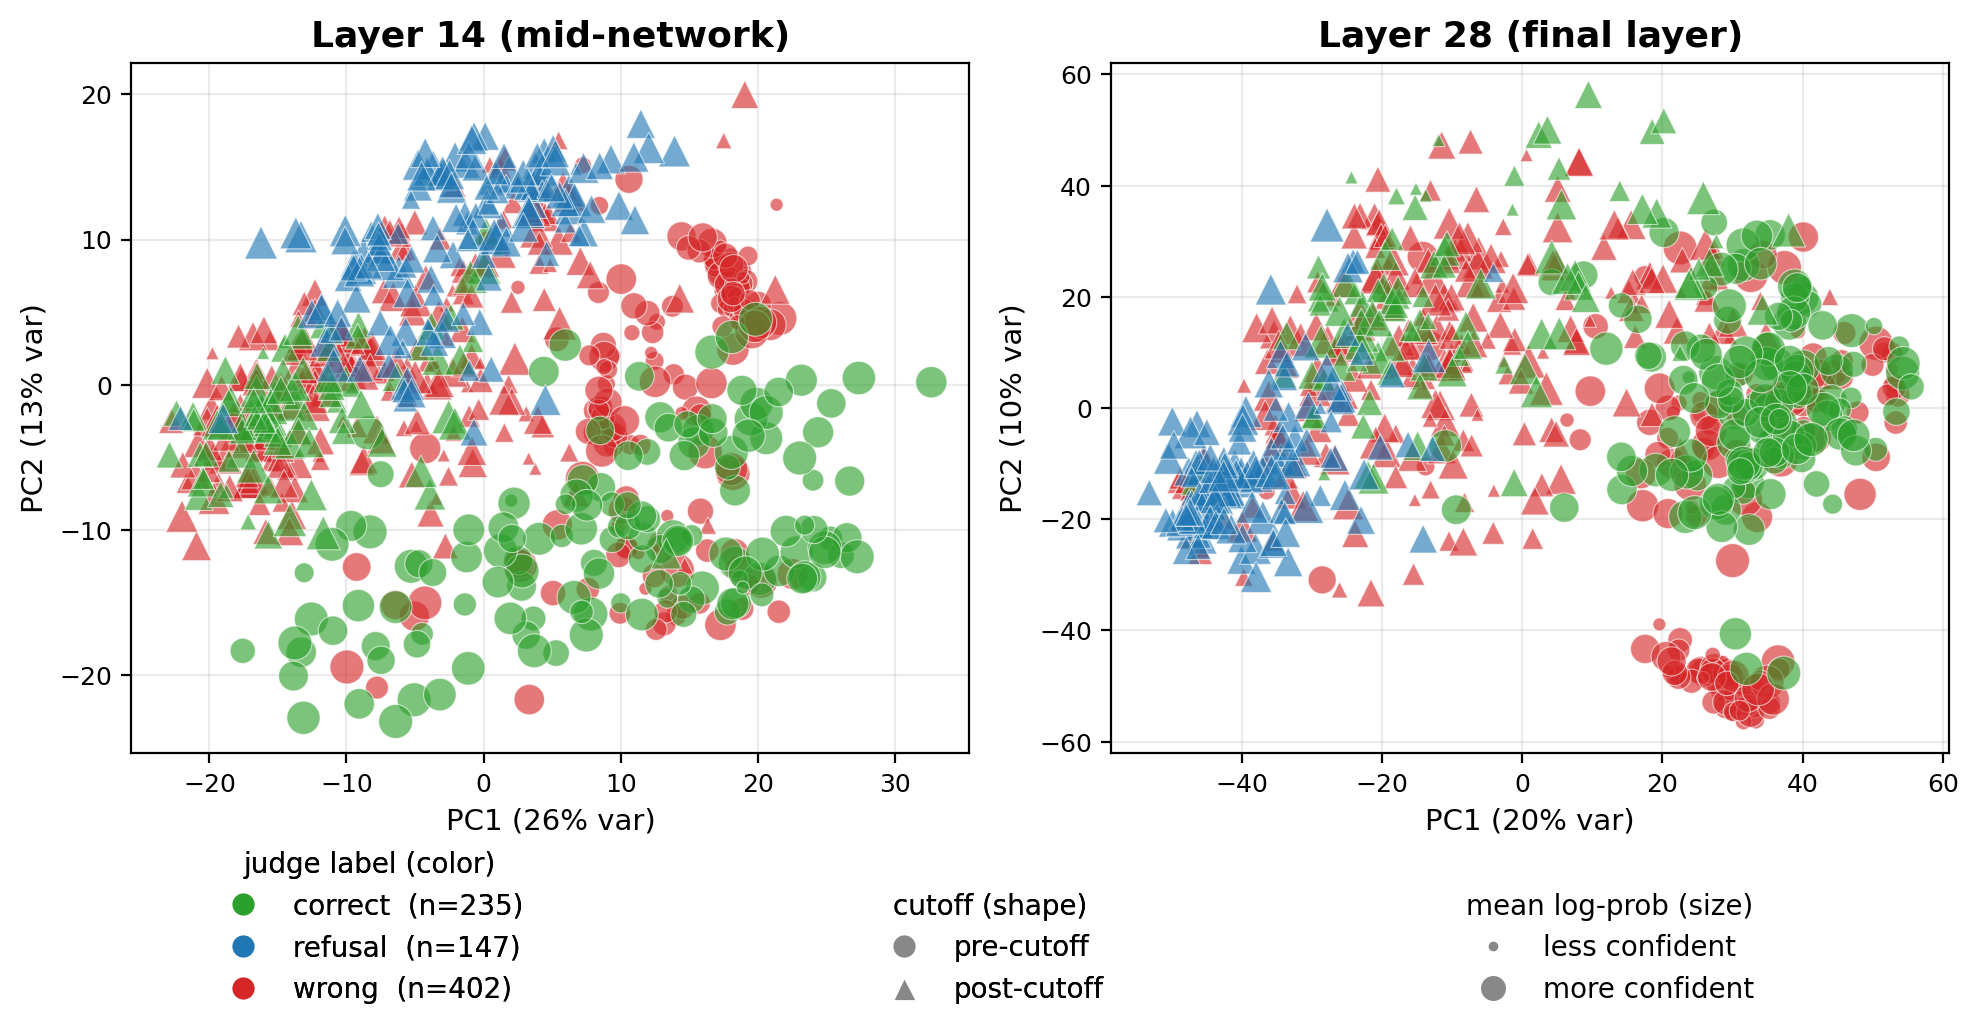
\includegraphics[keepaspectratio,alt={Hidden-state geometry, unsupervised.
  PCA(2) of the last-prompt-token hidden state at a mid-network layer (left) and the final
  layer (right), n=784. Each point is one question, encoded on three channels at once:
  color is the judge label (green correct, blue refusal, red wrong), marker shape is
  cutoff class (circle pre-cutoff, triangle post-cutoff), and marker size is the mean
  per-token log-probability (larger = more confident). At layer 14 the classes mix
  heavily; by layer 28 the refusals (blue, necessarily post-cutoff) pull into a distinct
  cluster with no supervision, the correct answers occupy the opposite side, and a tight
  group of large red markers (the confident confabulations of Section 5.3) separates out
  on its own. The refusal cluster is the geometry the refusal-vs-wrong probe
  reads.}]{figures/qwen3_1_7b/embeddings_pca_merged.png}}
\caption{Hidden-state geometry, unsupervised (Section 5.4). PCA(2) of
the last-prompt-token hidden state at a mid-network layer (left) and the
final layer (right), \(n=784\). Color is the judge label (green correct,
blue refusal, red wrong), marker shape is cutoff class (circle
pre-cutoff, triangle post-cutoff), marker size is the mean per-token
log-probability. At layer 14 the classes mix heavily; by layer 28 the
refusals (blue, necessarily post-cutoff) pull into a distinct cluster
with no supervision, the correct answers occupy the opposite side, and a
tight group of large red markers (the confident confabulations of
Section 5.3) separates out on its own.}\label{fig:embeddings}
\end{figure}

\subsubsection{A.5 Probe-peak summary vs.~majority
baselines}\label{a.5-probe-peak-summary-vs-majority-baselines}

\begin{table}[!htbp]
\small
\centering
\caption{Hidden-state probe vs.~the four prompt-feature baselines; ``h
adds'' = probe peak \(-\) strongest (bolded)
baseline.\label{tbl:hadds}}
\begin{tabular}{@{}
  >{\raggedright\arraybackslash}p{(\linewidth - 14\tabcolsep) * \real{0.4940}}
  >{\raggedleft\arraybackslash}p{(\linewidth - 14\tabcolsep) * \real{0.0723}}
  >{\raggedleft\arraybackslash}p{(\linewidth - 14\tabcolsep) * \real{0.0723}}
  >{\raggedleft\arraybackslash}p{(\linewidth - 14\tabcolsep) * \real{0.0723}}
  >{\raggedleft\arraybackslash}p{(\linewidth - 14\tabcolsep) * \real{0.0723}}
  >{\raggedleft\arraybackslash}p{(\linewidth - 14\tabcolsep) * \real{0.0723}}
  >{\raggedleft\arraybackslash}p{(\linewidth - 14\tabcolsep) * \real{0.0723}}
  >{\raggedleft\arraybackslash}p{(\linewidth - 14\tabcolsep) * \real{0.0723}}@{}}
\toprule
\begin{minipage}[b]{\linewidth}\raggedright
target
\end{minipage} & \begin{minipage}[b]{\linewidth}\raggedleft
majority
\end{minipage} & \begin{minipage}[b]{\linewidth}\raggedleft
TF-IDF
\end{minipage} & \begin{minipage}[b]{\linewidth}\raggedleft
text-only
\end{minipage} & \begin{minipage}[b]{\linewidth}\raggedleft
+domain
\end{minipage} & \begin{minipage}[b]{\linewidth}\raggedleft
+category
\end{minipage} & \begin{minipage}[b]{\linewidth}\raggedleft
\textbf{hidden state}
\end{minipage} & \begin{minipage}[b]{\linewidth}\raggedleft
\textbf{h adds}
\end{minipage} \\\midrule
\texttt{correct} & 0.700 & 0.767 & 0.773 & 0.779 & \textbf{0.800} &
\(0.824\) & \(+2.4\) \\
\texttt{cutoff} & 0.622 & 0.940 & \textbf{0.952} & 0.952 & 1.000\textsuperscript{$\dagger$} &
\(0.982\) & \(+3.0\) \\
\texttt{refusal\_vs\_wrong} & 0.732 & \textbf{0.820} & 0.803 & 0.805 &
0.800 & \(0.894\) & \(\mathbf{+7.4}\) \\
\texttt{refusal\_vs\_wrong}\texttt{\_within\_post} & 0.626 &
\textbf{0.774} & 0.741 & 0.730 & 0.730 & \(0.870\) &
\(\mathbf{+9.6}\) \\
\texttt{correct\_within\_pre} & 0.527 & 0.797 & 0.811 & 0.811 &
\textbf{0.818} & \(0.848\) & \(+3.0\) \\
\texttt{correct\_within}\texttt{\_obscure} & 0.667 & 0.752 &
\textbf{0.830} & 0.811 & 0.811 & \(0.805\) & \(-2.5\) \\
\bottomrule
\end{tabular}
\end{table}


Table \ref{tbl:probepeaks} is the Section 5.5 probe-peak summary
(vs.~majority baseline only).

\begin{table}[!htbp]
\small
\centering
\caption{Probe peaks vs.~majority baselines (Qwen3-1.7B,
ConfabQA).\label{tbl:probepeaks}}
\begin{tabular}{@{}
  >{\raggedright\arraybackslash}p{(\linewidth - 12\tabcolsep) * \real{0.4487}}
  >{\raggedleft\arraybackslash}p{(\linewidth - 12\tabcolsep) * \real{0.0641}}
  >{\raggedleft\arraybackslash}p{(\linewidth - 12\tabcolsep) * \real{0.0641}}
  >{\raggedright\arraybackslash}p{(\linewidth - 12\tabcolsep) * \real{0.0897}}
  >{\raggedleft\arraybackslash}p{(\linewidth - 12\tabcolsep) * \real{0.1795}}
  >{\raggedleft\arraybackslash}p{(\linewidth - 12\tabcolsep) * \real{0.0769}}
  >{\raggedleft\arraybackslash}p{(\linewidth - 12\tabcolsep) * \real{0.0769}}@{}}
\toprule
\begin{minipage}[b]{\linewidth}\raggedright
target
\end{minipage} & \begin{minipage}[b]{\linewidth}\raggedleft
n
\end{minipage} & \begin{minipage}[b]{\linewidth}\raggedleft
best layer
\end{minipage} & \begin{minipage}[b]{\linewidth}\raggedright
1\(\sigma\) layer range
\end{minipage} & \begin{minipage}[b]{\linewidth}\raggedleft
peak acc
\end{minipage} & \begin{minipage}[b]{\linewidth}\raggedleft
majority
\end{minipage} & \begin{minipage}[b]{\linewidth}\raggedleft
margin
\end{minipage} \\\midrule
\texttt{correct} (all items) & 784 & 18 & 10--28 & \(0.824 \pm 0.031\) &
0.700 & \(+12.4\) \\
\texttt{cutoff} (all items) & 784 & 13 & 10--20 & \(0.982 \pm 0.005\) &
0.622 & \(+36.0\) \\
\texttt{refusal\_vs\_wrong} & 549 & 28 & 16--28 & \(0.894 \pm 0.019\) &
0.732 & \(+16.2\) \\
\texttt{refusal\_vs\_wrong\_within\_post} & 393 & 28 & 20--28 &
\(0.870 \pm 0.022\) & 0.626 & \(+24.4\) \\
\texttt{correct\_within\_pre} & 296 & 18 & 9--28 & \(0.848 \pm 0.038\) &
0.527 & \(+32.1\) \\
\texttt{correct\_within\_obscure} & 153 & 7 & 1--28 &
\(0.805 \pm 0.063\) & 0.667 & \(+13.8\) \\
\bottomrule
\end{tabular}
\end{table}

The 1\(\sigma\) layer-range column matters: for the within-obscure probe
at n=153, accuracies across the entire 28-layer network are within one
fold-standard-deviation of the argmax, so the specific ``peak layer 7''
is not a meaningful per-depth claim; only the overall mean accuracy is.

% ----- B. Prompts, schemas, and data artifacts -----
\subsection{B. Prompts, schemas, and data
artifacts}\label{b.-prompts-schemas-and-data-artifacts}

\subsubsection{B.1 Judge prompt}\label{b.1-judge-prompt}

The full judge system prompt and template are in \texttt{judge.py}. The
system prompt defines a three-way decision rule (\texttt{CORRECT} /
\texttt{REFUSAL} / \texttt{WRONG}), gives five worked few-shot examples,
and instructs the model to emit exactly one line of the form
\texttt{Label:\ X}; the parser is a regex on
\texttt{Label:\textbackslash{}s*(CORRECT\textbar{}REFUSAL\textbar{}WRONG)}. The user-message template embeds the question, the
gold answer, the acceptable alternatives, and the model's answer in a
fixed quoted-block format. A regex parser extracts the label from the
judge output; on parse failure the fallback is to scan for a bare
keyword on the first line, then to label as \texttt{wrong} with a
\texttt{parse\_error:\ true} field for audit.

\subsubsection{B.2 Validation prompt
schema}\label{b.2-validation-prompt-schema}

The validation prompt emitted by
\texttt{01\_question\_set.py\ -\/-emit-validation-prompt} is in
\texttt{data/questions\_v1\_validation\_prompt.md}; the JSON output
schema returned by the external LLM is specified in that file's
``Required output format'' section. The validation pipeline
(\texttt{01\_question\_set.py\ -\/-emit-validation-prompt}
-\textgreater{} external LLM -\textgreater{}
\texttt{-\/-apply-validation}) is reproducible bitwise from the source
files and validation results, and gold corrections leave an audit trail
in \texttt{validation\_notes}.

\textbf{A case study for the validation pipeline.} During an early
iteration of the benchmark the item \texttt{sci\_ob\_05} asked ``What is
the half-life of the muon, in microseconds?'' The gold, written by the
dataset author from memory, was \(2.197\), which is in fact the muon
\emph{mean lifetime} \(\tau_\mu\), not the half-life
\(t_{1/2} = \tau_\mu \ln 2 \approx 1.52\ \mu\text{s}\). The external
validation pass flagged this \(30.7\%\) systematic error; the source
question was subsequently rewritten to ask explicitly for the mean
lifetime, eliminating the ambiguity. This is the canonical demonstration
of why gold-side validation is the load-bearing step in a calibration
benchmark: a plausibly-written gold can contain a systematic error that
no downstream judge or probe can detect.

The Section 3 obscure item in full: ``Who won the Academy Award for
Best Actor at the 1968 ceremony for `In the Heat of the Night'?''
(gold: Rod Steiger).

\subsubsection{B.3 Annotator-agreement data for judge
calibration}\label{b.3-annotator-agreement-data-for-judge-calibration}

Two independent annotators re-graded ConfabQA alongside the Qwen3-1.7B
judge; Table \ref{tbl:judge} summarizes the agreement.

\begin{table}[!htbp]
\small
\centering
\caption{Judge agreement on ConfabQA across three
annotators.\label{tbl:judge}}
\begin{tabular}{@{}
  >{\raggedright\arraybackslash}p{(\linewidth - 8\tabcolsep) * \real{0.5897}}
  >{\raggedleft\arraybackslash}p{(\linewidth - 8\tabcolsep) * \real{0.0897}}
  >{\raggedleft\arraybackslash}p{(\linewidth - 8\tabcolsep) * \real{0.1410}}
  >{\raggedleft\arraybackslash}p{(\linewidth - 8\tabcolsep) * \real{0.0897}}
  >{\raggedleft\arraybackslash}p{(\linewidth - 8\tabcolsep) * \real{0.0897}}@{}}
\toprule
\begin{minipage}[b]{\linewidth}\raggedright
pair
\end{minipage} & \begin{minipage}[b]{\linewidth}\raggedleft
items
\end{minipage} & \begin{minipage}[b]{\linewidth}\raggedleft
agree
\end{minipage} & \begin{minipage}[b]{\linewidth}\raggedleft
rate
\end{minipage} & \begin{minipage}[b]{\linewidth}\raggedleft
Cohen's \(\kappa\)
\end{minipage} \\\midrule
DR vs.~Qwen-judge (full ConfabQA) & \(784\) & \(682 / 784\) & \(87.0\%\)
& \(0.780\) \\
Claude vs.~Qwen-judge (stratified 30-item sample) & \(30\) & \(30 / 30\)
& \(100\%\) & \(1.000\) \\
\bottomrule
\end{tabular}
\end{table}

The annotation sources:

\begin{itemize}
\tightlist
\item
  \texttt{data/gemini\_regrade/qwen3\_1\_7b\_dr\_labels.jsonl}: DR
  (Gemini 3.1 Pro with web-search verification) grading all \(784\)
  items using the literal \texttt{judge.py} three-way decision rule.
\item
  \texttt{data/claude\_grading\_v1.json}: Claude Opus 4.7 grading a
  stratified \(30\)-item sample (\texttt{random.Random(42)}, 10 items
  per category) from (\texttt{question}, \texttt{gold},
  \texttt{model\ answer}) triples under the same rule.
\end{itemize}

Cohen's \(\kappa\) corrects the raw agreement rate for the agreement two
annotators would reach by chance:

\begin{equation}
\kappa \;=\; \frac{p_o - p_e}{1 - p_e},
\label{eq:kappa}
\end{equation}

where \(p_o\) is the observed agreement rate and \(p_e\) is the rate
expected if the two annotators labeled independently with their observed
marginal label distributions. For DR vs.~the Qwen-judge on all \(784\)
items, \(p_o = 682/784 = 0.870\) and \(p_e = 0.409\), giving
\(\kappa = 0.78\).

The \(102\) DR vs.~Qwen-judge disagreements decompose as \(45\) items DR
calls wrong where the Qwen-judge calls correct (Qwen too lenient on
partial-match containment), \(38\) DR-wrong / Qwen-refusal (DR sees
fabrication where Qwen sees hedging), \(11\) DR-refusal / Qwen-wrong,
\(7\) DR-correct / Qwen-wrong, and \(1\) DR-refusal / Qwen-correct.

The Qwen judge labels are embedded in the response files under
\texttt{data/responses/qwen3\_1\_7b/} (one \texttt{\{id\}.json} per
item). Agreement statistics for both annotators are in Table
\ref{tbl:judge}; the DR pass additionally web-verified each gold answer
and flagged three items with stated-premise errors
(\texttt{his\_pc\_09}: month wrong by one; \texttt{his\_pc\_56}: year
wrong by one; \texttt{his\_pc\_90}: dual premise error), flagged for
source patching in v2.

\textbf{DR strictness and label-sensitivity rerun (Section 4).} DR is
systematically stricter than the Qwen-judge (\(467\) vs.~\(402\)
wrong-labels), and the residual \(13\%\) disagreement primarily reflects
DR's stricter containment rule and independent gold verification, not
judge miscalibration. A sensitivity rerun under the DR labels keeps the
picture: the refusal-vs-wrong probe reaches \(87.1\%\) (vs.~\(89.4\%\)
under the judge labels; margin over a TF-IDF question-text baseline
\(+3.9\) vs.~\(+7.7\) pp), and the layer-18 correctness probe
\emph{rises} to \(87.6\%\) (margin \(+9.8\) vs.~\(+6.0\) pp); artifact
\texttt{revision\_analyses}. The three flagged stated-premise items
(\(3/784 \approx 0.4\%\)) are retained because dropping them does not
shift any headline number; v2 will patch them at the source.

\textbf{Regrade of intervened generations (Sections 4, 6).} The
intervened generations of Section 6 are graded by the subject model; a
blind Claude-family regrade of \(60\) of them agrees with the self-judge
at \(85\%\) (\(\kappa = 0.76\), comparable to the graders'
\(\kappa = 0.78\) on natural outputs), with disagreements balanced
across label directions rather than inflating flip rates (artifact
\texttt{intervened\_regrade\_claude}).

\subsubsection{B.4 Authoritative
summary}\label{b.4-authoritative-summary}

Every Qwen3-1.7B single-model number in Sections 5.1--5.6 and 6.1--6.2
is derived from \texttt{data/qwen3\_1\_7b\_summary.json}, generated by
\texttt{03\_analyze.py} in a single pass over the cached responses and
activations. The summary file records: per-judge, per-cutoff,
per-category, and per-domain counts; full per-layer accuracy curves and
1\(\sigma\) layer ranges for every probe target; class-imbalance metrics
at peak for the refusal probe; and all three prompt-feature baseline
variants. Reproducing those numbers consists of running
\texttt{python\ 03\_analyze.py} and reading the resulting JSON. The
Section 6 and Sections 7--8 numbers are recorded in per-experiment
artifacts under \texttt{figures/}, one JSON (with the generating script
of the same name under \texttt{analysis/} or \texttt{saes/}) per
experiment: \texttt{13\_intervention\_results},
\texttt{14\_intervention\_correct\_subset},
\texttt{15\_intervention\_three\_directions},
\texttt{16\_intervention\_random\_controls},
\texttt{intervention\_dose\_ratios}, \texttt{revision\_analyses},
\texttt{small\_cell\_stats}, \texttt{intervened\_regrade\_claude},
\texttt{17\_intervention\_gemma\_subnorm},
\texttt{correctness\_direction\_lens},
\texttt{correctness\_direction\_intervention},
\texttt{refusal\_direction\_meandiff}, \texttt{pca\_coverage\_2191},
\texttt{probe\_2191\_blend}, \texttt{sae\_decompose\_prenorm},
\texttt{optimized\_refusal\_direction}, \texttt{sae\_causal\_ablation},
\texttt{sae\_feature\_refusal\_rate},
\texttt{sae\_apology\_feature\_test},
\texttt{sae\_feature\_trajectories}, \texttt{sae\_wrong\_features},
\texttt{prefix\_forcing\_control}, \texttt{hidden\_state\_norms},
\texttt{bootstrap\_h\_adds}, \texttt{bootstrap\_llama\_external},
\texttt{bootstrap\_qwen3\_4b}, \texttt{refusal\_channel\_test}, and
\texttt{cross\_dataset\_transfer\_\textless{}model\textgreater{}}. The
Section 6.3 scripts read the pre-norm activation cache, rebuilt with
\texttt{python\ -m\ analysis.cache\_prenorm\_states} (Appendix D.2).

\subsubsection{B.5 Sample source-file
entry}\label{b.5-sample-source-file-entry}

\begin{verbatim}
data/sources/science/nobel_physics.json:
{
  "_documentation": {...},
  "template": "Who won the Nobel Prize in Physics in {year}?",
  "answer_field": "winner",
  "well_known": [...], "obscure": [...], "post_cutoff": [...]
}
\end{verbatim}

\subsubsection{B.6 Token-flow and baseline
schematics}\label{b.6-token-flow-and-baseline-schematics}

Figure \ref{fig:tokenflow} shows the two forward-pass regimes behind the
Section 2.2 probe target; Figure \ref{fig:pipeline} shows the Section
2.3 probe pipeline; Figure \ref{fig:baselines} sketches the Section 2.4
baseline design.

\textbf{Confidence metrics in full (Section 2.1).}
At each generation step \(t\) the model produces a distribution
\(p_t(\cdot)\) over the next token; all generation is greedy
(\texttt{do\_sample=False}, hence deterministic), so the emitted token
is the mode of \(p_t\). Two scalar summaries of the generated response
recur in §5, both means over the \(T_g\) generated positions
(\(t = T, \ldots, T+T_g-1\), with \(T\) the prompt length and
\(T_g \le 64\)):

\begin{equation}
\bar\ell = \frac{1}{T_g} \sum_{t=T}^{T+T_g-1} \ell_t,
\quad \ell_t = \log \max_{x \in \mathcal{V}} p_t(x);
\qquad
\bar H = \frac{1}{T_g} \sum_{t=T}^{T+T_g-1} H_t,
\quad H_t = -\sum_{x \in \mathcal{V}} p_t(x) \log p_t(x).
\label{eq:lbar}
\end{equation}

In \eqref{eq:lbar}, \(\ell_t\) is the log-probability of the emitted
(argmax) token, so \(\bar\ell\) is the length-normalized answer
likelihood: \(\exp(\bar\ell)\) is the geometric mean of the per-token
probabilities, and \(\bar\ell = -0.05\) corresponds to \(\approx 0.95\)
per token (I also report \(\min_t \ell_t\) as a worst-step diagnostic).
\(H_t\) is the Shannon entropy of \(p_t\) in nats
(\(\approx 0\) when near-deterministic, \(\log|\mathcal{V}|\) when
uniform); \(\bar\ell\) scores the picked token, \(\bar H\) the whole
distribution, and the two are tightly anti-correlated empirically
(Figure \ref{fig:confidence}b, Appendix A.2).
 The last-prompt-position prefill state is the natural
probe target for three reasons: \textbf{causal masking}
(\(h^{(\ell)}_T\) summarizes the whole prompt, and no later prompt
position adds information); \textbf{output-locality} (\(h^{(L)}_T\) as
cached, the final normed state of Section 4, is up to a linear
projection the first answer token's logit vector, so anything linearly
decodable from it is available to the output head at the moment of
commitment); and \textbf{no generation contamination} (probing
\emph{generated} tokens' states conflates what the model knows with what
it has already committed to saying, since the generated prefix is fed
back as input). On the Section 2.1 metrics: \(\bar\ell\) and \(\bar H\)
can come apart when one dominant mass carries a long thin tail of
plausible alternatives.

\begin{figure}
\centering
% Per-layer probe pipeline (split from the old 3-panel methods figure).
\begin{tikzpicture}[
  font=\footnotesize,
  >={Stealth[length=2mm]},
  node distance=4mm and 5mm,
  databox/.style = {draw=orange!75!black, fill=orange!8, rounded corners=2pt,
                    inner sep=4pt, align=center},
  opbox/.style   = {draw=blue!60!black,   fill=blue!6,   rounded corners=2pt,
                    inner sep=4pt, align=center},
  outbox/.style  = {draw=green!50!black,  fill=green!8,  rounded corners=2pt,
                    inner sep=4pt, align=center},
  basebox/.style = {draw=violet!60!black, fill=violet!8, rounded corners=2pt,
                    inner sep=4pt, align=center},
  arr/.style     = {->, semithick, gray!50!black},
]

\node [databox, text width=2.6cm] (slice) at (0,0)
       {Slice at layer $\ell$\\$X\in\mathbb{R}^{n\times d}$};

\node [opbox, right=5mm of slice]  (scaler) {StandardScaler};
\node [opbox, right=3mm of scaler] (pca)    {PCA(16)};
\node [opbox, right=3mm of pca]    (lr)     {LogReg};
\node [outbox, right=5mm of lr, text width=2.5cm] (cv)
      {Stratified\\5-fold CV};

\draw [arr] (slice)  -- (scaler);
\draw [arr] (scaler) -- (pca);
\draw [arr] (pca)    -- (lr);
\draw [arr] (lr)     -- (cv);

\node [databox, below=4mm of slice.south west, anchor=north west,
       text width=12.2cm, align=left] (targets)
      {Probe targets $y\in\{0,1\}$:\hspace{1em}
       correct\hspace{1em}$\cdot$\hspace{1em}cutoff (pre/post)\hspace{1em}$\cdot$\hspace{1em}%
       refusal-vs-wrong\hspace{1em}$\cdot$\hspace{1em}correct-within-pre};

\end{tikzpicture}

\caption{Per-layer linear-probe pipeline. At each layer $\ell$, the $n \times d$ matrix
of captured hidden states is passed through StandardScaler $\to$ PCA(16) $\to$ logistic
regression and evaluated with stratified 5-fold CV, separately for each binary target.}
\label{fig:pipeline}
\end{figure}

\begin{figure}
\centering
% Token flow: conventional autoregressive generation vs. the prefill pass.
\begin{tikzpicture}[
  font=\footnotesize,
  >={Stealth[length=2mm]},
  node distance=4mm and 5mm,
  databox/.style = {draw=orange!75!black, fill=orange!8, rounded corners=2pt,
                    inner sep=4pt, align=center},
  opbox/.style   = {draw=blue!60!black,   fill=blue!6,   rounded corners=2pt,
                    inner sep=4pt, align=center},
  outbox/.style  = {draw=green!50!black,  fill=green!8,  rounded corners=2pt,
                    inner sep=4pt, align=center},
  arr/.style     = {->, semithick, gray!50!black},
  lbl/.style     = {font=\scriptsize\itshape, text=gray!40!black, align=center},
  panel/.style   = {font=\scriptsize\bfseries, anchor=south west},
]

% ---- (a) conventional autoregressive generation ----
\node [databox, text width=2.6cm] (aprompt) at (0,0)
      {prompt tokens\\$x_1 \ldots x_T$};
\node [opbox, right=6mm of aprompt, text width=2.3cm] (alm)
      {LM forward\\pass};
\node [outbox, right=6mm of alm, text width=2.9cm] (adist)
      {$p_t(\cdot)$ over $\mathcal{V}$\\$\to$ next token};
\node [databox, right=6mm of adist, text width=2.5cm] (aout)
      {answer tokens\\$x_{T+1} \ldots x_{T+T_g}$};
\draw [arr] (aprompt) -- (alm);
\draw [arr] (alm) -- (adist);
\draw [arr] (adist) -- (aout);
\draw [arr, dashed] (aout.south) .. controls +(-0.2,-0.9) and +(0.2,-0.9) .. (alm.south);
\node [lbl, below=10mm] at ($(alm.south)!0.5!(aout.south)$)
      {each emitted token is appended to the input:\\one forward pass per generated token};
\node [panel] at ($(aprompt.north west)+(0,1mm)$) {(a) conventional generation};

% ---- (b) prefill pass ----
\node [databox, text width=2.6cm, below=27mm of aprompt] (bprompt)
      {prompt tokens\\$x_1 \ldots x_T$};
\node [opbox, right=6mm of bprompt, text width=2.3cm] (blm)
      {LM forward\\pass (prefill)};
\node [outbox, right=6mm of blm, text width=5.2cm] (bh)
      {last-prompt-token hidden states $h^{(\ell)}_T$\\
       $\ell = 0 \ldots L$: one $(L{+}1) \times d$ tensor};
\draw [arr] (bprompt) -- (blm);
\draw [arr] (blm) -- (bh);
\node [lbl, below=2.5mm] at ($(blm.south)!0.5!(bh.south)$)
      {single forward pass over the prompt; nothing generated yet};
\node [panel] at ($(bprompt.north west)+(0,1mm)$) {(b) prefill pass};

\end{tikzpicture}

\caption{Token flow in the two forward-pass regimes. \textbf{(a)} Conventional
generation runs one forward pass per generated token, feeding each emitted token back
into the input. \textbf{(b)} The prefill pass stops just before the first generated
token; the hidden state at that moment, $h^{(\ell)}_T$, is saved at every layer $\ell$
and is what the probes read. Generation starts from exactly this state, so it is the
model's representation immediately before it commits to an answer; stacked over
questions it forms the probe input tensor $(n,\ L{+}1,\ d) = (784,\ 29,\ 2048)$. The
dimensions ($L{=}28$, $d{=}2048$) are specific to Qwen3-1.7B; the other subject models
differ in both depth and width.}
\label{fig:tokenflow}
\end{figure}

\begin{figure}
\centering
% Baselines (split from the old 3-panel methods figure).
\begin{tikzpicture}[
  font=\footnotesize,
  >={Stealth[length=2mm]},
  node distance=4mm and 5mm,
  databox/.style = {draw=orange!75!black, fill=orange!8, rounded corners=2pt,
                    inner sep=4pt, align=center},
  opbox/.style   = {draw=blue!60!black,   fill=blue!6,   rounded corners=2pt,
                    inner sep=4pt, align=center},
  outbox/.style  = {draw=green!50!black,  fill=green!8,  rounded corners=2pt,
                    inner sep=4pt, align=center},
  basebox/.style = {draw=violet!60!black, fill=violet!8, rounded corners=2pt,
                    inner sep=4pt, align=center},
  arr/.style     = {->, semithick, gray!50!black},
]

\node [basebox, text width=5.0cm] (maj) at (0,0)
      {Majority baseline\\$\max\!\big(P(y{=}1),\ P(y{=}0)\big)$};

\node [basebox, right=6mm of maj, text width=6.4cm] (txt)
      {Prompt-text classifier\\TF-IDF~+~LR on question text\\
       \footnotesize (+~engineered features,~domain,~category)};

\node [below=4mm of maj.south west, anchor=north west,
       text width=12.2cm, align=center,
       font=\small\bfseries] (verdict)
       {Probe is evidence of model-internal information \emph{iff}
        probe acc.\ $>$ max(both baselines).};

\node [below=1mm of verdict.south, anchor=north,
       text width=12.2cm, align=center, font=\footnotesize\itshape]
       {$h_{\rm adds}$ = probe peak $-$ strongest baseline (pp).};

\end{tikzpicture}

\caption{Baselines, fit on the same labels with no access to the hidden state: the
majority class, and a prompt-text classifier, TF-IDF (term-frequency /
inverse-document-frequency bag-of-words) plus logistic regression, with engineered
features and domain/category dummies. A probe is evidence of model-internal information
only insofar as it beats both; $h_{\rm adds}$ = probe peak $-$ strongest baseline (pp),
reported throughout \S\S5--8.}
\label{fig:baselines}
\end{figure}

\subsubsection{B.7 Prompt-feature baseline
specification}\label{b.7-prompt-feature-baseline-specification}

Formal Section 4 target definitions: \texttt{correct} is binary
\texttt{judge\_label\ ==\ "correct"}; \texttt{cutoff} is binary
\texttt{cutoff\_class\ ==\ "post"}; \texttt{refusal\_vs\_wrong} is
binary \texttt{judge\_label\ ==\ "refusal"} on the
\texttt{\{refusal,\ wrong\}} subset; the within-post and within-stratum
variants restrict the item pool as named.

On the Section 2.3 probe pipeline: with \(n = 784\) items and
\(d = 2048\) features, a raw logistic regression would massively
overfit; projecting onto the top 16 principal directions first keeps the
ratio of training items to fitted parameters at \(\approx 19{:}1\)
instead of \(\approx 0.15{:}1\) (\texttt{C} is sklearn's inverse
regularization strength, at its default), and \texttt{sklearn.Pipeline}
semantics fit scaler and PCA on the training fold only.

The four Section 4 baselines in full:

\begin{itemize}
\tightlist
\item
  \textbf{TF-IDF} (term frequency--inverse document frequency):
  \texttt{TfidfVectorizer} (\texttt{ngram\_range=(1,2)},
  \texttt{min\_df=2}, \texttt{max\_df=0.95},
  \texttt{sublinear\_tf=True}) \(\to\)
  \texttt{LogisticRegression(max\_iter=2000,\ C=1.0)} on the raw
  question text: the strongest ``what could a bag-of-tokens classifier
  learn'' baseline.
\item
  \textbf{text-only (engineered)}: numeric features only (question
  character length, word count, has-year indicator, year value, number
  of capitalized words, digits, commas, ends-with-\texttt{?} indicator).
\item
  \textbf{text + domain}: engineered features plus domain one-hot.
\item
  \textbf{text + domain + category}: adds the human-assigned category
  dummy, the annotator's expected-difficulty label; for the
  \texttt{cutoff} target it is excluded from the strongest-baseline
  comparison (Section 4).
\end{itemize}

% ----- C. Intervention calibration and details -----
\subsection{C. Intervention calibration and
details}\label{c.-intervention-calibration-and-details}

Calibration and supporting detail for the Section 6.2, Section 6.3.1,
and Section 7.2 one-shot interventions.

\textbf{Magnitude and normalization.} Magnitude enters only as a mixing
ratio. Spelled out, with \(\mathrm{rms}(x) = \|x\|/\sqrt{d}\) and
\(\mathrm{RMSNorm}(x) = \mathbf{g} \odot x / \mathrm{rms}(x)\), the
intervened head input is

\[\mathrm{RMSNorm}(h + \alpha\hat{\mathbf{w}})
  \;=\; \frac{\sqrt{d}\; \mathbf{g} \odot (h + \alpha\hat{\mathbf{w}})}
  {\sqrt{\|h\|^{2} + 2\alpha \langle h, \hat{\mathbf{w}} \rangle + \alpha^{2}}},\]

which depends only on the ratios \(\alpha / \|h\|\) and
\(\langle h, \hat{\mathbf{w}} \rangle / \|h\|\) and converges to
\(\mathrm{RMSNorm}(\pm\hat{\mathbf{w}})\) as \(\alpha \to \pm\infty\).
Here \(h\) is the post-block-27 residual, the state the hook actually
perturbs: its norm across all \(784\) items is \(1640 \pm 220\)
(\(\mathrm{rms}(h) \approx 36\)), so the single \(\overline{\|h\|}\)
used in the alpha-translation below describes typical items to within
\(\sim 15\%\). One structured feature: refusal states are markedly
tighter (\(1636 \pm 89\), a \(5\%\) coefficient of variation) than
correct (\(1665 \pm 312\)) or wrong (\(1627 \pm 184\)) states; the
templated behavior is geometrically stereotyped as well
(\texttt{figures/qwen3\_1\_7b/hidden\_state\_norms.json} records both
this and the final normed state's statistics). The lens scores are
therefore the asymptote of the first-token dose-response, which is the
saturation Sections 6.2 and 6.3.1 observe, and why \(\alpha\) ranges
must be calibrated to each model's hidden-state scale (Table
\ref{tbl:scales}). The clean asymptotic story holds only when the hook
feeds the final RMSNorm directly; when it sits below the final layer
(Gemma at layer 19, the layer-18 correctness intervention), later blocks
process the perturbed state, and large \(|\alpha|\) is genuinely
off-manifold rather than asymptotic, the pathology Appendix C records.

\textbf{Choice of \(\alpha\) scale, in full (Qwen3-1.7B).} The natural
scale is much larger than the per-fold projection variance because
RMSNorm dampens the perturbation: the post-norm contribution to the LM
head is approximately
\(\mathbf{d} \cdot W_{\mathrm{LM}}^\top / \mathrm{RMS}(\mathbf{h})\),
and at the intervention point \(\mathrm{RMS}(\mathbf{h}) \approx 36\).
Empirically, on a pre-cutoff probe item the natural greedy first token
loses to the refusal opener \texttt{As} at \(\alpha \approx 2000\), and
at \(\alpha = 5000\) the top six tokens are entirely refusal openers;
the sweep covers this range. In relatable units: baseline states already
lean toward the direction (mean \(\cos = +0.36\) on refusal items,
\(+0.10\) on wrong, at \(\overline{\|h\|} \approx 1640\)), and the
sweep \(\alpha \in \{-2000, -500, +500, +1500, +3000\}\) corresponds
to mean perturbation-to-state-norm ratios
\(\{1.23, 0.31, 0.31, 0.92, 1.84\}\times\) and mean post-intervention
alignments \(\{-.73, -.13, +.43, +.74, +.90\}\) (averaged over the
\(n=549\) subset). Per item, on the actual intervention subsets
(artifact \texttt{intervention\_dose\_ratios}): \(\pm 500\) is
sub-norm for every pushed item (ratio \(\le 0.39\)), the saturating
\(+1500\) sits at the state's own norm (wrong-subset ratio
\(0.96 \pm 0.09\); a third of items exceed \(1\times\)), and
\(\pm(2000\)--\(3000)\) is super-norm (\(\approx 1.9\times\)) for
all. The smallest effective dose \(\alpha = +500\) reaches only
\(0.43\) alignment yet already flips half the first tokens.

\textbf{Hook and opener set (Section 6.2).} The intervention hook sits
on \texttt{model.model.layers{[}27{]}}, whose output is the
post-block-27 residual feeding the final RMSNorm; the pushed vector is
the unit-normalized within-post recovery (the full-subset recovery is a
substantially different vector, cosine \(0.33\)). The first-token
opener set is \{ \texttt{as}, \texttt{as}, \texttt{As}, \texttt{作为},
\texttt{作為}, \texttt{作为一个}, \texttt{There}, \texttt{there} \}.

\textbf{Coordinate dissociation: normed vs.~pre-norm recovery (Section
6.2).} Refitting the same probe pipeline natively on the pre-norm
residuals dissociates the two roles of the direction: the native
recovery reads the class split equally well (\(88.9\%\) vs.\
\(89.4\%\) CV accuracy) but is a substantially different vector
(cosine \(0.49\) to the normed-space recovery) with half the causal
leverage (\(41\%\) vs.~\(92\%\) held-out first-token flips at the
\(0.9\times\) dose; artifact \texttt{revision\_analyses}).

\textbf{Steering-matrix parity block (Section 6.2).} Table
\ref{tbl:alphaparity} repeats the Table \ref{tbl:alpha} protocol with
the SAE-2191 and directly optimized directions on the same items
(per-direction opener rates saturate by \(+0.3\times\);
Table~\ref{tbl:threedirs}); the \(0\) column is the shared unperturbed
baseline. Wrong items reach the same one-in-three judged-refusal
plateau (already at \(+0.3\times\), matching the steeper first-token
curves of Table~\ref{tbl:threedirs}), de-refused items land as
confabulations at the same rates, and correct items survive the pull
while largely resisting the push (artifacts in Appendix B.4).

\begin{table}[!htbp]
\small
\centering
\caption{Steering-matrix parity: the Table \ref{tbl:alpha} protocol
rerun with the SAE-2191 and directly optimized directions on the same
items (story metric per subset; doses as fractions of the mean pre-norm
state norm).\label{tbl:alphaparity}}
\begin{tabular}{@{}llrrrrrr@{}}
\toprule
original label & metric & $-1.2\times$ & $-0.3\times$ & $0$ & $+0.3\times$ & $+0.9\times$ & $+1.8\times$ \\
\midrule
WRONG & judged REFUSAL (2191) & $7\%$ & $3\%$ & $0\%$ & $30\%$ & $27\%$ & $23\%$ \\
 & judged REFUSAL (optim.) & $13\%$ & $13\%$ & $0\%$ & $30\%$ & $30\%$ & $30\%$ \\
REFUSAL & judged WRONG (2191) & $67\%$ & $70\%$ & $0\%$ & $0\%$ & $0\%$ & $23\%$ \\
 & judged WRONG (optim.) & $77\%$ & $77\%$ & $0\%$ & $0\%$ & $0\%$ & $0\%$ \\
CORRECT & judged CORRECT (2191) & $97\%$ & $100\%$ & $100\%$ & $60\%$ & $50\%$ & $77\%$ \\
 & judged CORRECT (optim.) & $90\%$ & $93\%$ & $100\%$ & $50\%$ & $50\%$ & $50\%$ \\
\bottomrule
\end{tabular}
\end{table}

\textbf{Random-direction controls (Sections 6.2, 6.3.1).} Three
norm-matched random directions and a shuffled-label probe direction, run
through the identical generate-and-judge protocol (artifact
\texttt{16\_intervention\_random\_controls}), leave the steering matrix
unmoved at the sub-norm dose. At \(\alpha = -500\) the controls keep
\(29\)--\(30/30\) refusals refusing (vs.~\(6\)--\(12/30\) under the
three real directions), and at \(+500\)--\(+1500\) they yield
\(\le 13\%\) judged refusals and \(\le 40\%\) opener rates on wrong
items (vs.~\(27\)--\(30\%\) and \(97\)--\(100\%\)). One of the three
random seeds does partially collapse refusals at the super-norm
\(-2000\) dose (\(16/30\) wrong): super-norm doses can act by magnitude
alone, which is why the working regime is kept at or below the state
norm.

\textbf{Optimized-direction training details (Section 6.3).} The
optimized refusal direction treats the intervention vector
\(\mathbf{v}\) as the only trainable parameter and maximizes the mean
log-probability of the refusal-opener token set under the final RMSNorm
and LM head, on a train half of the \(402\) wrong pre-norm states, with
\(\|\mathbf{v}\|\) fixed at a sub-nudge \(0.12\times\) dose (no
full-model backpropagation needed). The optimum lands next to feature
2191: cosine \(0.64\) to the feature's decoder vector, against \(0.22\)
to the Section 6.2 probe direction and \(0.25\) to the mean difference,
and its logit lens is a pure opener cone (\texttt{As}, \texttt{As},
\texttt{\_as}, \texttt{"As}).

\textbf{Feature 2191 dose-response table.} The full sweep behind the
Section 6.3.1 ablation:

\begin{table}[!htbp]
\small
\centering
\caption{Feature 2191 dose-response: next-token refusal-opener
probability under
\(\alpha \cdot \hat W_{\rm dec}[2191]\).\label{tbl:dose}}
\begin{tabular}{@{}
  >{\raggedleft\arraybackslash}p{(\linewidth - 6\tabcolsep) * \real{0.2500}}
  >{\raggedleft\arraybackslash}p{(\linewidth - 6\tabcolsep) * \real{0.2500}}
  >{\raggedleft\arraybackslash}p{(\linewidth - 6\tabcolsep) * \real{0.2500}}
  >{\raggedleft\arraybackslash}p{(\linewidth - 6\tabcolsep) * \real{0.2500}}@{}}
\toprule
\begin{minipage}[b]{\linewidth}\raggedleft
\(\alpha\)
\end{minipage} & \begin{minipage}[b]{\linewidth}\raggedleft
wrong: \(P(\rm opener)\)
\end{minipage} & \begin{minipage}[b]{\linewidth}\raggedleft
wrong: argmax-in-opener
\end{minipage} & \begin{minipage}[b]{\linewidth}\raggedleft
refusal: \(P(\rm opener)\)
\end{minipage} \\\midrule
\(0\) & \(0.000\) & \(0/30\) & \(0.969\) \\
\(16\) & \(0.000\) & \(0/30\) & \(0.981\) \\
\(64\) & \(0.000\) & \(0/30\) & \(0.998\) \\
\(200\) & \(0.000\) & \(0/30\) & \(1.000\) \\
\(400\) & \(\mathbf{0.364}\) & \(\mathbf{11/30}\) & \(1.000\) \\
\(750\) & \(\mathbf{1.000}\) & \(\mathbf{30/30}\) & \(1.000\) \\
\(1500\) & \(1.000\) & \(30/30\) & \(1.000\) \\
\(3000\) & \(1.000\) & \(30/30\) & \(1.000\) \\
\bottomrule
\end{tabular}
\end{table}

\textbf{Norm accounting for the probe--2191 pair.} The component of
\(\mathbf{w}_{\rm raw}\) along feature 2191 has length
\(0.16\,\|\mathbf{w}_{\rm raw}\|\), the relevant scale for logit
contributions, which are linear in the component; the orthogonal
remainder keeps \(0.99\,\|\mathbf{w}_{\rm raw}\|\) (in the additive
Pythagorean accounting, energy shares of \(2.6\%\) vs \(97.4\%\)). Two
nearly disjoint vectors produce the same first-token flip because the
flip requires only a sufficient projection onto the opener unembedding
cone after RMSNorm; at the causal level the probe direction acts through
its \(0.16\)-of-norm component.

\begin{table}[!htbp]
\small
\centering
\caption{First-token refusal-opener rate on \(201\) held-out wrong
items under pushes along the three candidate refusal directions, doses
as fractions of the mean state norm (bfloat16 final-norm{+}head
evaluation; the optimized direction is trained on the other half of the
wrong items at the \(0.12\times\) dose. The probe direction's fit pool
included these \(201\) items, an asymmetry that favors the probe and
so cannot explain its lower curve).\label{tbl:threedirs}}
\begin{tabular}{@{}lrrrrrrr@{}}
\toprule
direction & \(0.03\times\) & \(0.06\times\) & \(0.12\times\) & \(0.21\times\) & \(0.30\times\) & \(0.46\times\) & \(0.91\times\) \\
\midrule
probe (Section 6.2) & \(13\%\) & \(17\%\) & \(22\%\) & \(29\%\) & \(35\%\) & \(45\%\) & \(92\%\) \\
SAE feature 2191 & \(20\%\) & \(27\%\) & \(40\%\) & \(64\%\) & \(91\%\) & \(100\%\) & \(100\%\) \\
directly optimized & \(22\%\) & \(34\%\) & \(54\%\) & \(97\%\) & \(100\%\) & \(100\%\) & \(100\%\) \\
\bottomrule
\end{tabular}
\end{table}

\textbf{Dose-for-dose potency.} \textbf{Which ``as'' direction is more
potent?} The two interventions are directly comparable: both add a
unit-norm vector, so \(\alpha\) is the added norm in both sweeps, and
both score the same statistic, the first-token argmax landing in the
opener set (on different \(30\)-item wrong subsets). Their half-flip
doses are similar: the probe direction reaches \(50\%\) at
\(\alpha = 500\); feature 2191 is at \(11/30\) by \(\alpha = 400\) and
completes \(30/30\) by \(750\), where the probe needs \(1500\) for
\(97\%\). The concentrated feature saturates roughly twice as early. The
naive projection accounting, under which the probe direction owns only \(0.25\) of its norm on the 2191 channel and should need \(\approx 4\times\) the dose, overstates the gap: the probe's remaining
norm is not opener-inert, since it also pushes the broader opener family
(\texttt{there}, the Chinese variants) that the flip criterion counts,
and the flip is a competition threshold rather than a linear readout.

By the strict judge criterion the comparison is exact, since all the
causal routes were run on the same \(30\) wrong items (Section 6.3.1).
The probe direction converts \(30\%\) into judged refusals at
\(\alpha = +1500\), forcing the literal token ``As'' converts \(37\%\),
forcing ``No'' converts \(27\%\), and feature 2191 converts \(30\%\) at
\(\alpha = 750\) and \(27\%\) at \(1500\). Every route to the opener
token produces the same downstream refusal rate of roughly one in three,
consistent with complete mediation at the first token (each route
\(n=30\); the comparison is not powered as an equivalence test).
Released as
\texttt{figures/qwen3\_1\_7b/sae\_feature\_refusal\_rate.json}
(\texttt{analysis/sae\_feature\_refusal\_rate.py}).

\textbf{Apology-feature push (Section 6.3).} Adding
\(\alpha \cdot \hat W_{\rm dec}[14034]\) at the Section 6.2 intervention
point, at the same doses that saturate feature 2191 (\(\alpha = 750\),
\(1500\)), produces zero \texttt{Sorry}/\texttt{Oops} openers in \(60\)
generations; the feature's causal output routes through its weaker
\texttt{There} component instead (\(13/30\) There-openers at
\(\alpha = 1500\), and all eight induced judged refusals open with
``There'').

\textbf{Correctness-direction null: protocol, rates, and flip forensics
(Section 6.2).} The Section 6.2 one-shot protocol applied to the
layer-18 correctness direction (\(\alpha \in [-3000, +3000]\), \(n=30\)
originally-correct and \(n=30\) originally-wrong items).
Originally-correct items degrade mildly at large
\(|\alpha|\) in \emph{both} directions (\(100\% \to 80\)--\(83\%\)
correct at \(\alpha = \mp 3000\)), originally-wrong items flip to
correct at low, sign-independent rates (\(17\%\) at both \(-3000\) and
\(+3000\)), and refusal induction is scattered (\(0\)--\(17\%\)) with no
dose-response. The flips concentrate on a recurring handful of items
rather than spreading across the subset: the union over all six nonzero
\(\alpha\) is \(10\) of \(30\) items, five account for most flips, and
one flips at every nonzero \(\alpha\) in both directions. Inspection
shows these are items where the correct answer was already marginally
available, a knife-edge wrong decode of a famous fact, or a
post-cutoff fact the model demonstrably knows but hedges on, so a kick
of any sign can dislodge the default trajectory. This null is in
tension with inference-time intervention reports of
truthfulness-direction steering \citep{li2023iti}; the settings differ
(TruthfulQA's misconception-heavy distribution, multi-head attention
interventions, and a truthful-vs-untruthful contrast rather than
correct-vs-wrong recall), and reconciling them is future work.

\textbf{Hidden-state scales.} The per-model scale statistics and
calibrated \(\alpha\) ranges below. In perturbation-to-state-norm units
the swept ranges are not comparable across models: \(\le 1.8\times\)
the state norm for Qwen (\(\alpha = 3000\) on
\(\overline{\|h\|} = 1640\)), \(\approx 25\times\) for Gemma
(\(\alpha = 8000\) on its mid-network residual scale of \(326\);
the sub-norm rerun of Section 7.2 shows the directional effect does
not depend on that regime), and
\(\approx 8\times\) for Llama (\(\alpha = 300\) on a remeasured
residual scale of \(39\)). The Llama sweep therefore never probed the
sub-norm regime at all, which is consistent with its
magnitude-dominated behavior (Table~\ref{tbl:llamasweep} discussion):
its directional evidence should be revisited at
\(\alpha \approx \pm 20\)--\(40\). The Qwen and Llama rows below are
the pre-norm residuals the interventions actually perturb (the earlier
draft quoted final-normed-state norms); Gemma's mid-network hook was
cached correctly:

\begin{table}[!htbp]
\small
\centering
\caption{Per-model state scale at the intervention hook (Qwen, Llama:
post-block residual feeding the final norm, remeasured; Gemma:
post-block-19 residual as cached) and the calibrated \(\alpha\)
ranges.\label{tbl:scales}}
\begin{tabular}{@{}lrrrl@{}}
\toprule
model & hook layer & \(\overline{\|h\|}\) & \(\sigma_{\|h\|}\) & \(\alpha\) swept \\
\midrule
Qwen3-1.7B & 28 & \(1640\) & \(220\) & \([-2000, +3000]\) \\
Gemma 2 2B & 19 & \(326\) & \(16\) & \([-6000, +8000]\) \\
Llama 3.2 3B & 28 & \(39\) & \(3.8\) & \([-300, +300]\) \\
\bottomrule
\end{tabular}
\end{table}

\textbf{Qwen3-1.7B sample generations (Section 6.2).}
(\texttt{cin\_pc\_60}, gold ``Jacques Audiard''; baseline says ``Luis
Llosa'', a confabulation):

\begin{center}
\small
\begin{tabular}{@{}
  >{\raggedleft\arraybackslash}p{(\linewidth - 2\tabcolsep) * \real{0.5000}}
  >{\raggedright\arraybackslash}p{(\linewidth - 2\tabcolsep) * \real{0.5000}}@{}}
\toprule
\begin{minipage}[b]{\linewidth}\raggedleft
\(\alpha\)
\end{minipage} & \begin{minipage}[b]{\linewidth}\raggedright
first 100 chars
\end{minipage} \\\midrule
\(0\) &
\texttt{\textquotesingle{}Emilia\ Perez\textquotesingle{}\ (2024),\ a\ Spanish-language\ musical\ crime\ film,\ was\ directed\ by\ **Luis\ Llosa**.} \\
\(+1500\) &
\texttt{As\ of\ 2024,\ the\ Spanish-language\ musical\ crime\ film\ **"Emilia\ Perez"**\ was\ directed\ by\ **Miguel\ Ángel\ Martínez**.} \\
\(+3000\) & (same as \(+1500\)) \\
\bottomrule
\end{tabular}
\end{center}

And \texttt{cin\_pc\_34} (baseline refuses on the 2024 Venice Golden
Lion):

\begin{center}
\small
\begin{tabular}{@{}
  >{\raggedleft\arraybackslash}p{(\linewidth - 2\tabcolsep) * \real{0.5000}}
  >{\raggedright\arraybackslash}p{(\linewidth - 2\tabcolsep) * \real{0.5000}}@{}}
\toprule
\begin{minipage}[b]{\linewidth}\raggedleft
\(\alpha\)
\end{minipage} & \begin{minipage}[b]{\linewidth}\raggedright
first 100 chars
\end{minipage} \\\midrule
\(0\) &
\texttt{As\ of\ my\ knowledge\ cutoff\ in\ 2024,\ there\ is\ no\ official\ announcement\ regarding\ a\ director\ winning\ the\ Golden\ Lion...} \\
\(-500\) &
\texttt{The\ 2024\ Venice\ Film\ Festival\ took\ place\ from\ September\ 2\ to\ 14,\ 2024.\ The\ Golden\ Lion,\ the\ highest\ award...} \\
\(-2000\) & (same as \(-500\)) \\
\bottomrule
\end{tabular}
\end{center}

\textbf{Prefix-forcing control (Section 6.2).} Generating the same
\(30\) wrong items with the literal opener ``As'' forced as the first
generated token and no hidden-state perturbation yields a \(37\%\)
judge-refusal rate (\(11/30\)), statistically indistinguishable from the
\(30\%\) the intervention reaches at \(\alpha = +1500\) and \(+3000\),
where its first-token opener rate is \(97\)--\(100\%\). Forcing ``No''
instead yields \(27\%\) judged refusals, with \(2/30\) items becoming
\emph{correct} (the forced negation occasionally cancels the
confabulation), so the roughly one-in-three downstream rate is stable
across opener choices. Released as
\texttt{figures/qwen3\_1\_7b/prefix\_forcing\_control.json} and
\texttt{prefix\_forcing\_control\_no.json}
(\texttt{analysis/prefix\_forcing\_control.py}, \texttt{-\/-prefix}
selects the opener).

\textbf{Gemma 2 2B (\(n=30 + 30\), judge = Qwen3).}

\begin{table}[!htbp]
\small
\centering
\caption{Gemma 2 2B one-shot intervention across its calibrated
\(\alpha\) sweep (\(n = 30\) per subset; judge =
Qwen3-1.7B).\label{tbl:gemmasweep}}
\begin{tabular}{@{}
  >{\raggedright\arraybackslash}p{(\linewidth - 12\tabcolsep) * \real{0.4828}}
  >{\raggedleft\arraybackslash}p{(\linewidth - 12\tabcolsep) * \real{0.0862}}
  >{\raggedleft\arraybackslash}p{(\linewidth - 12\tabcolsep) * \real{0.0862}}
  >{\raggedleft\arraybackslash}p{(\linewidth - 12\tabcolsep) * \real{0.0862}}
  >{\raggedleft\arraybackslash}p{(\linewidth - 12\tabcolsep) * \real{0.0862}}
  >{\raggedleft\arraybackslash}p{(\linewidth - 12\tabcolsep) * \real{0.0862}}
  >{\raggedleft\arraybackslash}p{(\linewidth - 12\tabcolsep) * \real{0.0862}}@{}}
\toprule
\begin{minipage}[b]{\linewidth}\raggedright
metric
\end{minipage} & \begin{minipage}[b]{\linewidth}\raggedleft
\(\alpha = -6000\)
\end{minipage} & \begin{minipage}[b]{\linewidth}\raggedleft
\(-2000\)
\end{minipage} & \begin{minipage}[b]{\linewidth}\raggedleft
\(0\)
\end{minipage} & \begin{minipage}[b]{\linewidth}\raggedleft
\(+2000\)
\end{minipage} & \begin{minipage}[b]{\linewidth}\raggedleft
\(+4000\)
\end{minipage} & \begin{minipage}[b]{\linewidth}\raggedleft
\(+8000\)
\end{minipage} \\\midrule
WRONG: judge says REFUSAL & \(23\%\) & \(40\%\) & \(0\%\) &
\(\mathbf{87\%}\) & \(67\%\) & \(57\%\) \\
WRONG: first-token opener & \(0\%\) & \(0\%\) & \(13\%\) &
\(\mathbf{100\%}\) & \(70\%\) & \(83\%\) \\
REFUSAL: judge says REFUSAL & \(80\%\) & \(93\%\) & \(100\%\) &
\(100\%\) & \(97\%\) & \(87\%\) \\
REFUSAL: first-token opener & \(0\%\) & \(0\%\) & \(53\%\) & \(100\%\) &
\(77\%\) & \(90\%\) \\
\bottomrule
\end{tabular}
\end{table}

The effect is non-monotonic at large positive \(\alpha\): \(+4000\) and
\(+8000\) drop the judge-refusal rate to \(67\%\) and \(57\%\)
respectively, even as the first-token-opener rate stays high. At those
magnitudes Gemma starts producing fluent-but-off-target openers
(``Formal announcements have not been made yet, but Marc Webb is not
directing any\ldots{}'') that the Qwen judge sometimes parses as
\texttt{wrong}. The negative-\(\alpha\) direction produces a different
pathology: \(\alpha = -2000\) generations begin with garbled non-English
tokens (Cyrillic ``\cyrtext{виправивши}'', French ``conseille''),
suggesting Gemma's refusal direction is partially entangled with
prompt-encoding stability and pushing in the opposite direction
off-manifold.

\textbf{Llama 3.2 3B.} The full Llama intervention sweep, displaced here
from Section 7.2 because Llama's near-saturated default refusal
(\(97.5\%\) of post-cutoff failures) leaves only \(n=12\) confabulating
items, which is insufficient for a clean directional-causal claim.

\textbf{Subset:} \(n=12\) wrong-post-cutoff + \(n=15\) refusal items.
Judge: Qwen3-1.7B. \textbf{Calibrated \(\alpha\) range:}
\(\{-300, -100, 0, +100, +300\}\), an order of magnitude smaller than
the Qwen3 and Gemma ranges, calibrated to where Llama's outputs remain
coherent; the post-block-27 residual has \(\|\mathbf{h}\| = 39 \pm 3.8\)
(Table \ref{tbl:scales}), so the swept range reaches \(\approx 8\times\)
the state norm and never entered the sub-norm regime.

\begin{table}[!htbp]
\small
\centering
\caption{Llama 3.2 3B intervention over its calibrated \(\alpha\) range
(\(n=12\) wrong, \(n=15\) refusal
items).\label{tbl:llamasweep}}
\begin{tabular}{@{}
  >{\raggedright\arraybackslash}p{(\linewidth - 10\tabcolsep) * \real{0.1667}}
  >{\raggedleft\arraybackslash}p{(\linewidth - 10\tabcolsep) * \real{0.1667}}
  >{\raggedleft\arraybackslash}p{(\linewidth - 10\tabcolsep) * \real{0.1667}}
  >{\raggedleft\arraybackslash}p{(\linewidth - 10\tabcolsep) * \real{0.1667}}
  >{\raggedleft\arraybackslash}p{(\linewidth - 10\tabcolsep) * \real{0.1667}}
  >{\raggedleft\arraybackslash}p{(\linewidth - 10\tabcolsep) * \real{0.1667}}@{}}
\toprule
\begin{minipage}[b]{\linewidth}\raggedright
metric
\end{minipage} & \begin{minipage}[b]{\linewidth}\raggedleft
\(\alpha = -300\)
\end{minipage} & \begin{minipage}[b]{\linewidth}\raggedleft
\(-100\)
\end{minipage} & \begin{minipage}[b]{\linewidth}\raggedleft
\(0\)
\end{minipage} & \begin{minipage}[b]{\linewidth}\raggedleft
\(+100\)
\end{minipage} & \begin{minipage}[b]{\linewidth}\raggedleft
\(+300\)
\end{minipage} \\\midrule
WRONG: judge says REFUSAL & \(83\%\) & \(0\%\) & \(0\%\) & \(8\%\) &
\(75\%\) \\
WRONG: first-token opener & \(0\%\) & \(100\%\) & \(100\%\) & \(83\%\) &
\(0\%\) \\
REFUSAL: judge says REFUSAL & \(80\%\) & \(100\%\) & \(100\%\) &
\(100\%\) & \(93\%\) \\
REFUSAL: first-token opener & \(0\%\) & \(100\%\) & \(100\%\) & \(93\%\)
& \(0\%\) \\
\bottomrule
\end{tabular}
\end{table}

The wrong-subset row at the baseline (\(\alpha=0\)) reads \(0\%\)
refusal but \(100\%\) first-token-opener: items where the text reads
refusal-y (``I'm not aware of\ldots{}'') but commits mid-generation
(``\ldots However, I can tell you that\ldots{}''); the Qwen judge labels
these wrong because of the commit. The symmetric large-\(|\alpha|\)
refusal-rate spike (\(83\%\) at \(\alpha=-300\), \(75\%\) at
\(\alpha=+300\)) reflects the model producing shorter, judge-accepted
refusal-coded text but without using its standard opener vocabulary
(first-token-opener collapses to \(0\%\) in either direction). This is a
perturbation-magnitude effect, not a directional refusal-direction
causal signal.

The cleanest directional signal is the refusal subset at
\(\alpha = -300\): refusal rate drops from \(100\%\) to \(80\%\), three
of fifteen previously-refusing items committing to a confabulation:

\begin{center}
\small
\begin{tabular}{@{}
  >{\raggedright\arraybackslash}p{(\linewidth - 6\tabcolsep) * \real{0.2500}}
  >{\raggedright\arraybackslash}p{(\linewidth - 6\tabcolsep) * \real{0.2500}}
  >{\raggedright\arraybackslash}p{(\linewidth - 6\tabcolsep) * \real{0.2500}}
  >{\raggedright\arraybackslash}p{(\linewidth - 6\tabcolsep) * \real{0.2500}}@{}}
\toprule
\begin{minipage}[b]{\linewidth}\raggedright
id
\end{minipage} & \begin{minipage}[b]{\linewidth}\raggedright
gold
\end{minipage} & \begin{minipage}[b]{\linewidth}\raggedright
baseline (\(\alpha=0\)) answer
\end{minipage} & \begin{minipage}[b]{\linewidth}\raggedright
\(\alpha=-300\) answer
\end{minipage} \\\midrule
cin\_pc\_10 & Deadpool \& Wolverine & ``I'm not aware of any information
about a Marvel film\ldots{}'' & ``X-Men '97'' \\
\bottomrule
\end{tabular}
\end{center}

(Two other flips have similar structure; full per-item answers are in
\texttt{figures/llama\_3\_2\_3b/13\_intervention\_results.json}.)

% ----- D. Robustness checks -----
\subsection{D. Robustness checks}\label{d.-robustness-checks}

\subsubsection{D.1 Robustness to PCA truncation
depth}\label{d.1-robustness-to-pca-truncation-depth}

The headline probe pipeline uses \texttt{PCA(n\_components=16)}.
Sweeping over \(\{4, 8, 16, 32, 48,
64\}\) at each target shows that the peak per-layer accuracies are
stable within a \(\le 5\) pp band across the sweep (Figure
\ref{fig:pca-robustness}):

\begin{figure}
\centering
\pandocbounded{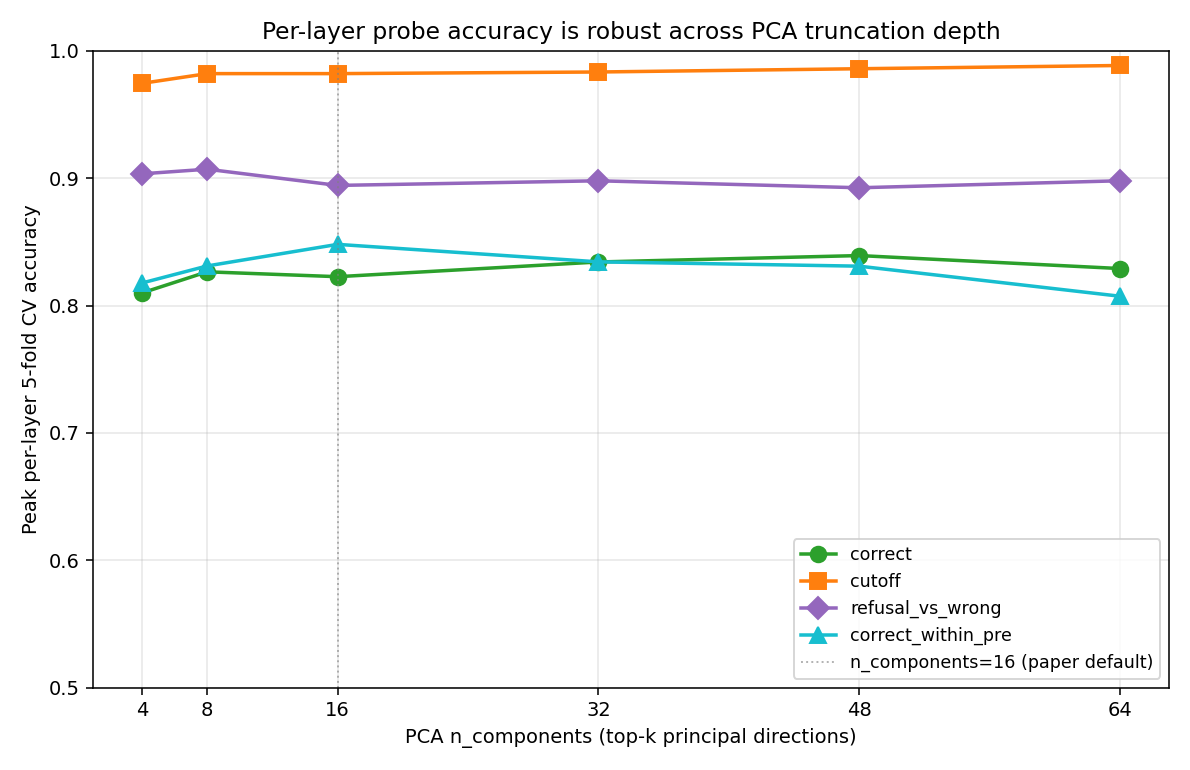
\includegraphics[keepaspectratio,alt={Peak per-layer probe accuracy as a
  function of PCA n\_\{\textbackslash mathrm\{components\}\}, for each of the main probe
  targets. The paper default (n=16) is marked. All targets are stable across the sweep
  within a \textbackslash le 5 pp band, and several peak at n \textbackslash ne 16, meaning
  the paper default is conservative rather than
  tuned.}]{figures/qwen3_1_7b/10_pca_robustness.png}}
\caption{Peak per-layer probe accuracy as a function of PCA
\(n_{\mathrm{components}}\), for each of the main probe targets. The
paper default (\(n=16\)) is marked. All targets are stable across the
sweep within a \(\le 5\) pp band, and several peak at \(n \ne 16\),
meaning the paper default is conservative rather than
tuned.}\label{fig:pca-robustness}
\end{figure}

The choice of \(n_{\mathrm{components}}=16\) is not driving any of the
reported numbers; the prompt-feature finding of Section 5.6 in
particular is independent of this hyperparameter. The full sweep data
(target \(\times\) \(n_{\mathrm{components}}\) peak-accuracy table) is
at \texttt{figures/qwen3\_1\_7b/10\_pca\_robustness.json}, generated by
\texttt{analysis/make\_robustness\_check.py}, which takes no arguments
and reads the same cached responses and activations as
\texttt{03\_analyze.py}.

\subsubsection{D.2 SAE base-to-instruct reconstruction
check}\label{d.2-sae-base-to-instruct-reconstruction-check}

Qwen-Scope was trained on Qwen3-1.7B-Base; the Section 6.3 subject is
the Instruct variant. The release declares its input contract
explicitly: hook \texttt{blocks.27.hook\_resid\_post} with
\texttt{normalize\_activations\ =\ none}, i.e.~the raw post-block-27
residual. On that state, recomputed over all \(549\) refusal+wrong items
via a live prefill hook (\texttt{analysis/cache\_prenorm\_states.py}),
the base\(\to\)instruct transfer is marginal by reconstruction quality:
per-item explained variance \(0.50\) (median \(0.51\)) and mean cosine
\(0.72\) (\texttt{figures/sae\_decompose\_prenorm.json}). An earlier
check (\texttt{saes/sae\_test\_reconstruction.py}) reported
\(\mathrm{EV}=0.82\)/cosine \(0.90\), but it was run at cached
hidden-states index \(24\), a different (post-block-23) residual, and
HF's cached index \(28\) is the final \emph{normed} state rather than
the declared hook (Section 4), so neither cached index measures the SAE
at its contract. The decisive validation of the Section 6.3 features is
therefore not reconstruction quality but the causal test of Section
6.3.1, which intervenes at the correct point and flips \(30/30\).

\subsubsection{D.3 PCA coverage and blend tests of feature
2191}\label{d.3-pca-coverage-and-blend-tests-of-feature-2191}

How much of feature 2191's decoder direction the probe's reachable
subspace can represent, and whether the feature can improve the probe's
split (Section 6.3). The dictionary that contains the feature was
estimated without ever seeing ConfabQA; that it nonetheless contains the
exact opener feature this benchmark activates is evidence 2191 is a
general unit of the model rather than an artifact of this question set.
Coverage: the pipeline's \(16\)-component subspace holds at most a
\(0.37\) cosine with \(\hat W_{\rm dec}[2191]\) (the recovered probe
sits at \(0.16\)); half coverage takes roughly \(60\) variance-ordered
components, and even the full \(549\)-dimensional span of the
benchmark's activations covers only \(0.79\). Blend: under 5-fold CV,
mixing the unit probe direction with the feature leaves the
refusal-vs-wrong AUC flat at \(0.944\) for mixing weights up to \(0.2\)
and degrades monotonically beyond, and a two-feature logistic stack over
both projections also lands at \(0.943\); the feature's out-of-subspace
mass carries no class information the probe has not already extracted.
The raw projection onto 2191 alone reaches AUC \(0.895\), close to the
probe's \(0.944\): the single dictionary direction carries nearly
probe-grade class information in the probed representation.

\subsubsection{D.4 Additional refusal-direction
diagnostics}\label{d.4-additional-refusal-direction-diagnostics}

\textbf{Score histograms (Section 6.1).} Figure \ref{fig:score-hist}
shows the signed projections of the layer-28 hidden states onto the
recovered refusal direction.

\begin{figure}
\centering
\pandocbounded{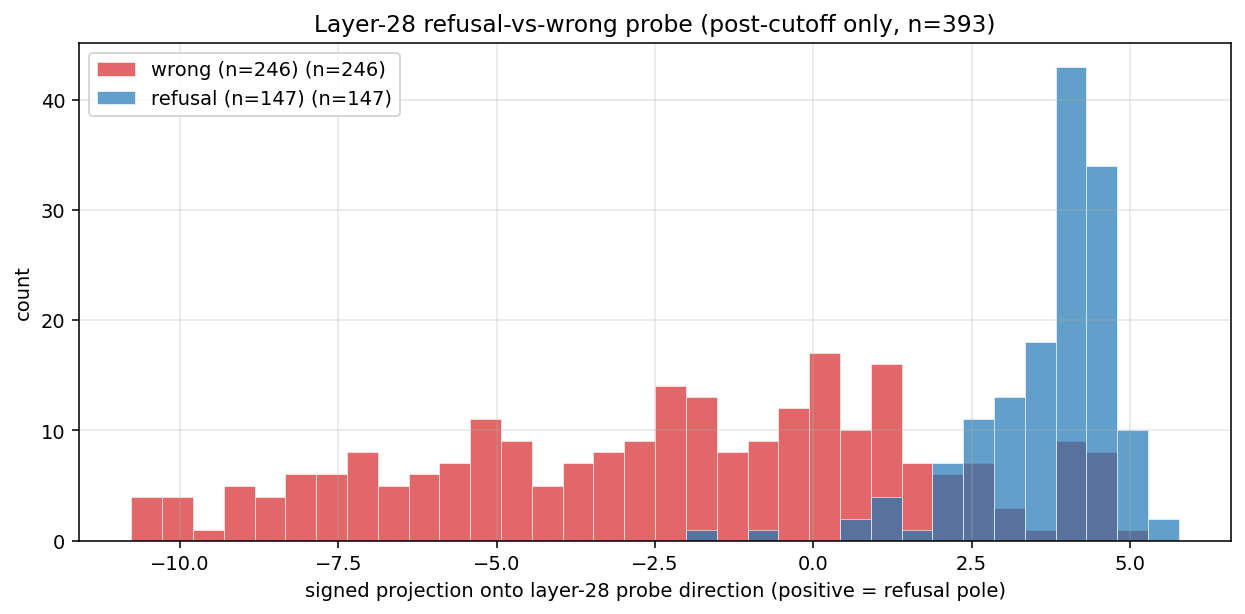
\includegraphics[keepaspectratio,alt={Score histogram: the signed
  projection of each item's layer-28 hidden state onto the recovered refusal direction, on
  the within-post subset (n = 393). Refusals concentrate at large positive projections;
  wrongs near zero or negative.}]{figures/qwen3_1_7b/12_probe_score_hist_refusal_vs_wrong_within_post.png}}
\caption{Score histogram: the signed projection of each item's layer-28
hidden state onto the recovered refusal direction, on the within-post
subset (\(n = 393\)). Refusals concentrate at large positive
projections; wrongs near zero or negative.}\label{fig:score-hist}
\end{figure}

\textbf{Refusal-direction lens scores (Section 6.1).} The lift
\((\mathbf{w}_{\mathrm{raw}})_i = (V^\top w)_i / \sigma_i\) is the
gradient of the probe score with respect to the raw state, the
hidden-state direction along which the score increases fastest; raw
units matter because the model's RMSNorm/LM head and the Section 6.2
intervention hook know nothing about the scaler. The lens scores are
relative alignment scores, not log-probabilities: with tied embeddings,
\(\ell_v = \langle \mathbf{e}_v, \mathbf{g} \odot \hat{\mathbf{w}} \rangle\)
(token row \(\mathbf{e}_v\), RMSNorm gain \(\mathbf{g}\),
\(\hat{\mathbf{w}}\) the direction divided by its root-mean-square).
Full subset (\(n=549\)): \texttt{as} leads at \(+19.22\), the Chinese refusal
openers \texttt{作为一个} and \texttt{作为} (``as'' / ``as a'') sit at
ranks 2--3 (\(+17.67\), \(+17.14\), with further variants at ranks
12--13), the rest of the top ten are case and spacing variants, and
\texttt{there} at rank 11 scores \(+14.16\). The within-post recovery's
lens yields the same vocabulary in a sharper form: '' as'' scores
\(+31.66\), ``作为'' \(+29.63\), ``\textbackslash tas'' \(+27.58\),
'' there'' \(+23.26\). The confabulation pole of the refusal direction
is dominated by generic low-frequency tokens with no thematic structure,
as expected: a confabulation can begin with any entity name, so there is
no concentrated ``confabulation vocabulary.'' The layer-18 correctness
direction under the same lens yields generic low-frequency fragments at
the correct pole and at most a faint uncertainty flavor (\texttt{不知}
``don't know'', \texttt{unknown}, \texttt{forgotten}) at the incorrect
pole.

\textbf{Recovery-method check: difference in class means (Section
6.1).} The raw difference of class means,
\(\bar{h}_{\mathrm{refusal}} - \bar{h}_{\mathrm{wrong}}\), at the same
layer is \emph{not} the probe direction: cosine \(0.46\) on the full
subset (\(0.36\) within post-cutoff, against a chance level of
\(\approx 0.02\) in \(2048\) dimensions), with only one of its top-ten
lens tokens (\texttt{as} itself, ranked first) overlapping the probe's.
Its lens instead mixes the opener with a temporal-currency vocabulary
(\texttt{current}, \texttt{currently}, \texttt{present}, \texttt{我没有}
``I don't have''), which dominates outright within post-cutoff. The two
recoveries weight different components: the mean difference absorbs
topical and temporal-currency content, the discriminatively trained
probe concentrates the register-and-opener component. A plain average of
refusal states, as a control, points at nothing but generic
sentence-starters (\texttt{As}, \texttt{The}, \texttt{There},
\texttt{In}).

Figure \ref{fig:geometry} shows the geometry behind the disagreement:
the mean difference is by construction the centroid connector, with
\(96\%\) of its norm in the top-two-PC plane where the wrong class's
covariance is widest, while the probe direction keeps only \(47\%\) of
its norm there, approximating instead the covariance-whitened difference
\(\Sigma^{-1}(\bar{h}_{\mathrm{refusal}} - \bar{h}_{\mathrm{wrong}})\)
that separates the classes item by item.


\textbf{The probe--2191 plane (Section 6.3.1).} Figure
\ref{fig:probe-sae-plane} shows the plane spanned by the probe refusal
direction and feature 2191's decoder vector.

\begin{figure}
\centering
\pandocbounded{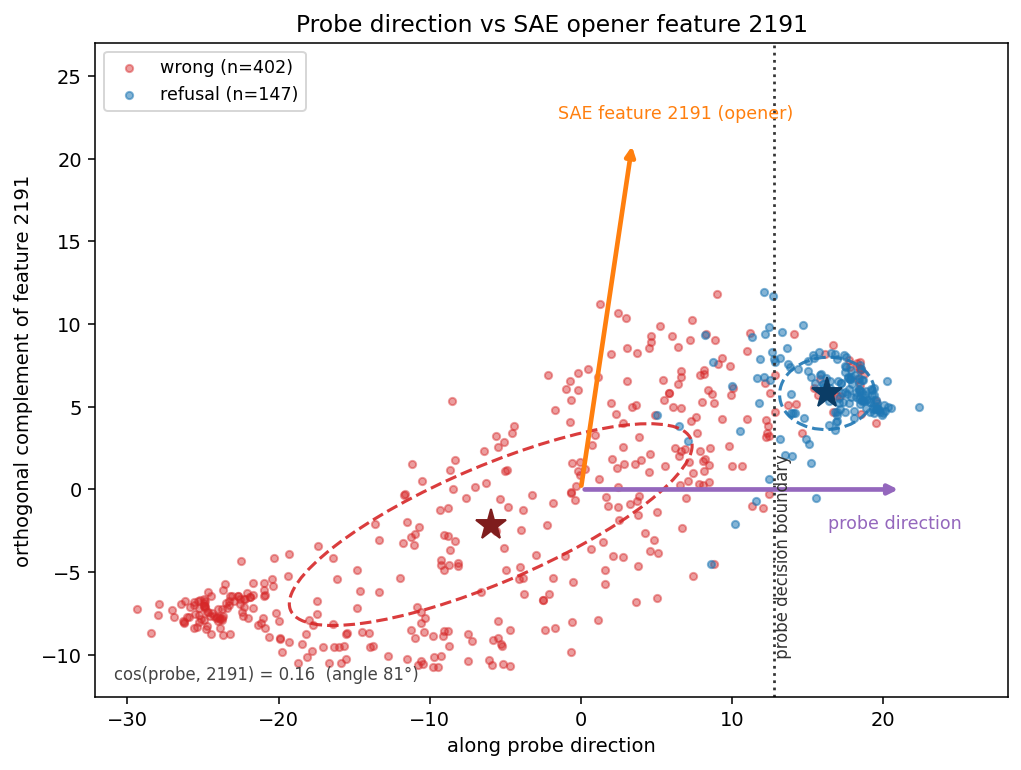
\includegraphics[keepaspectratio,alt={The plane spanned by the probe
  refusal direction and SAE feature 2191's decoder vector (refusal+wrong states in the
  probes' representation, n=549; stars: class centroids; dashed: per-class 1\textbackslash
  sigma covariance ellipses). The two arrows are 81\^{}\textbackslash circ apart (cosine
  0.16), yet the probe axis carries the class split and its decision boundary (dotted) is
  exact in this plane: a nearly probe-orthogonal output knob and a broad discriminative
  mixture share one causal channel. The optimized refusal direction is projected onto the
  same plane, drawn at its in-plane fraction (64 percent, angle to plane 50 degrees), and
  lands beside feature 2191.}]{figures/qwen3_1_7b/probe_sae_plane.png}}
\caption{The plane spanned by the probe refusal direction and SAE
feature 2191's decoder vector (refusal+wrong states in the probes'
representation, \(n=549\); stars: class centroids; dashed: per-class
\(1\sigma\) covariance ellipses). The two arrows are \(81^\circ\) apart
(cosine \(0.16\)), yet the probe axis carries the class split and its
decision boundary (dotted) is exact in this plane: a nearly
probe-orthogonal output knob and a broad discriminative mixture share
one causal channel. The optimized refusal direction (green, Section
6.3.1) is projected onto the same plane; its arrow is drawn at its
in-plane fraction, so its shorter length shows that \(64\%\) of it lies
in the plane (angle to plane \(50^\circ\)). It lands beside feature
2191 (cosine \(0.64\)), not the probe axis.}\label{fig:probe-sae-plane}
\end{figure}

\textbf{From h-space to a-space: what a push looks like in features
(Section 6.3).} The three views of Section 6.3 are static, and the
encoder \(a(h)\) is heavily nonlinear (TopK), so how an h-space push
maps into a-space is an empirical question. Figure
\ref{fig:feature-traj} tracks four ensemble members' mean activations on
the \(n=402\) wrong items as the post-block-27 residual is pushed along
the Section 6.2 direction and along \(\hat W_{\rm dec}[2191]\). Three
regularities emerge. First, 2191's activation grows smoothly and
linearly under both pushes (from its baseline of \(93\) on wrong items
to full coverage by \(\alpha \approx +1000\) on the probe push and
\(+200\) on its own), with a probe-to-2191 slope ratio of \(0.25\),
matching the two directions' cosine of \(0.25\): the TopK encoder is
locally linear along these rays. Second, the two pushes differ in what
else they recruit: the probe push feeds the whole register (17077 rises
to a mid-dose peak, 4314 grows steadily), while the pure 2191 push
crowds the hedge feature out entirely (4314 falls to \(0\) by
\(+3000\)). The probe direction moves wrong items \emph{toward}
refusal-like codes; the 2191 direction manufactures opener-dominated
ones; behaviorally the two are indistinguishable (Appendix C), so the
ensemble recruitment is not required for the flip. Third, the code as a
whole is substantially rewritten at behavioral doses: active-set overlap
with the unperturbed code falls to \(0.36\) (probe) and \(0.26\) (2191)
at \(\alpha=+1500\), and negative doses extinguish all four features.

\begin{figure}
\centering
\pandocbounded{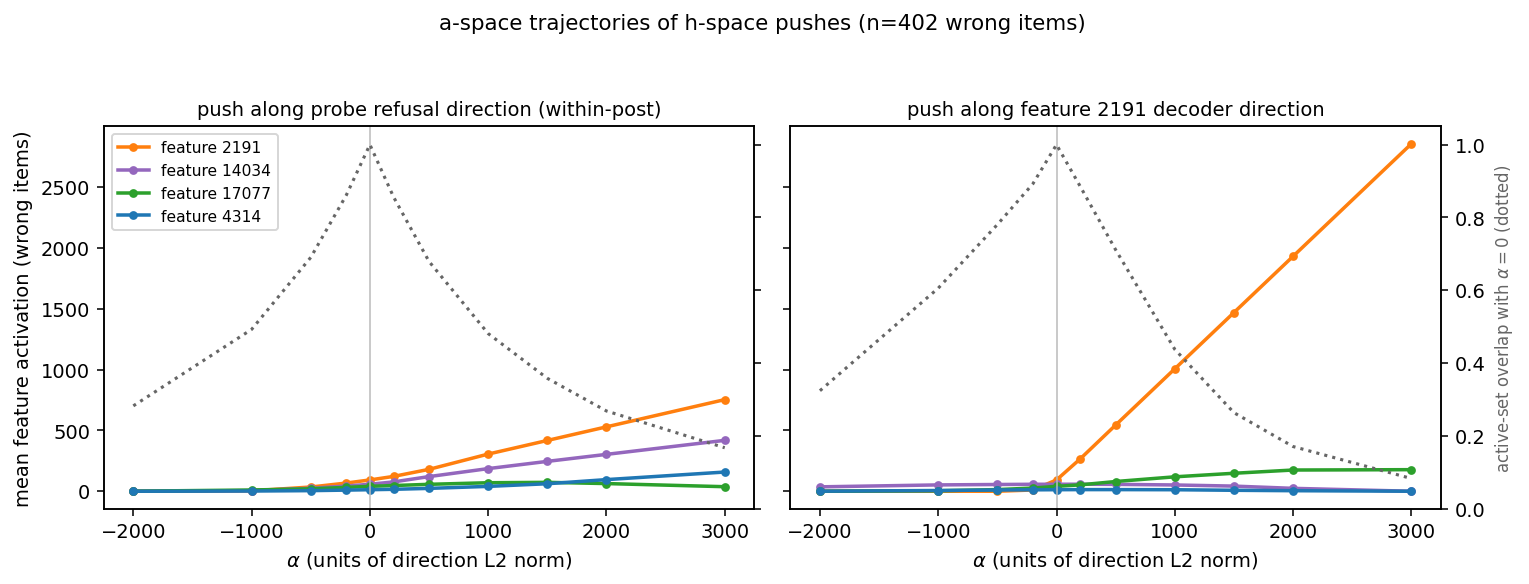
\includegraphics[keepaspectratio,alt={a-space trajectories of h-space
  pushes (n=402 wrong items, pre-norm residuals). Solid lines: mean activation of four
  ensemble features as the state is pushed along the Section 6.2 refusal direction (left)
  or feature 2191's decoder direction (right); dotted: mean overlap (Jaccard) of the
  active feature set with the unperturbed code. The probe push recruits the register
  broadly; the 2191 push concentrates on the opener and crowds out the
  hedge.}]{figures/qwen3_1_7b/sae_feature_trajectories.png}}
\caption{a-space trajectories of h-space pushes (\(n=402\) wrong items,
pre-norm residuals). Solid lines: mean activation of four ensemble
features as the state is pushed along the Section 6.2 refusal direction
(left) or feature 2191's decoder direction (right); dotted: mean overlap
(Jaccard) of the active feature set with the unperturbed code. The probe
push recruits the register broadly; the 2191 push concentrates on the
opener and crowds out the hedge.}\label{fig:feature-traj}
\end{figure}

\subsubsection{D.5 Cross-model comparison table and per-layer
probe curves}\label{d.5-cross-model-per-layer-probe-curves}

Table \ref{tbl:crossmodel} is the Section 7.1 cross-model comparison
summary. The correctness probe peaks in the same early-to-mid depth band
on all three architectures, but the absolute peaks hide the confound
Section 5.6 exposed: a large fraction of what looks like model-internal
correctness knowledge is the annotator-visible difficulty signal being
read back through the hidden state, and the margins remain modest within
the pre-cutoff stratum.

\begin{table}[!ht]
\small
\centering
\caption{Cross-model comparison
summary.\label{tbl:crossmodel}}
\begin{tabular}{@{}
  >{\raggedright\arraybackslash}p{(\linewidth - 6\tabcolsep) * \real{0.2500}}
  >{\raggedleft\arraybackslash}p{(\linewidth - 6\tabcolsep) * \real{0.2500}}
  >{\raggedleft\arraybackslash}p{(\linewidth - 6\tabcolsep) * \real{0.2500}}
  >{\raggedleft\arraybackslash}p{(\linewidth - 6\tabcolsep) * \real{0.2500}}@{}}
\toprule
\begin{minipage}[b]{\linewidth}\raggedright
Metric / Probe
\end{minipage} & \begin{minipage}[b]{\linewidth}\raggedleft
Qwen3-1.7B
\end{minipage} & \begin{minipage}[b]{\linewidth}\raggedleft
Gemma 2 2B
\end{minipage} & \begin{minipage}[b]{\linewidth}\raggedleft
Llama 3.2 3B
\end{minipage} \\\midrule
\textbf{Overall Accuracy} & 30.0\% & 31.9\% & 30.6\% \\
\textbf{Pre-cutoff Accuracy} & 47.3\% & 69.6\% & 80.7\% \\
\textbf{Post-cutoff Accuracy} & 19.5\% & 9.0\% & 0.2\% \\
\textbf{Refusal Rate on Post-cutoff Failures} & 37.4\% (147/393) &
55.2\% (245/444) & 97.5\% (475/487) \\
\midrule
\emph{Probe accuracies (peak \% {[}peak layer{]} vs baseline)} & & & \\
\textbf{Correctness (all items)} & \textbf{82.4\%} {[}L18{]}(base
70.0\%, +12.4 pp) & \textbf{89.7\%} {[}L14{]}(base 68.1\%, +21.6 pp) &
\textbf{94.3\%} {[}L13{]}(base 69.4\%, +24.9 pp) \\
\textbf{Cutoff (all items)} & \textbf{98.2\%} {[}L13{]}(base 62.2\%,
+36.0 pp) & \textbf{98.9\%} {[}L14{]}(base 62.2\%, +36.6 pp) &
\textbf{99.4\%} {[}L25{]}(base 62.2\%, +37.1 pp) \\
\textbf{Refusal-vs-Wrong (subset)} & \textbf{89.4\%} {[}L28{]}(base
73.2\%, +16.2 pp) & \textbf{83.9\%} {[}L19{]}(base 53.6\%, +30.3 pp) &
\textbf{95.8\%} {[}L28{]}(base 91.9\%, +3.9 pp) \\
\textbf{Correct within Pre-cutoff} & \textbf{84.8\%} {[}L18{]}(base
52.7\%, +32.1 pp) & \textbf{91.2\%} {[}L17{]}(base 69.6\%, +21.6 pp) &
\textbf{85.2\%} {[}L13{]}(base 80.7\%, +4.4 pp) \\
\textbf{Correct within Obscure} & \textbf{80.5\%} {[}L7{]}(base 66.7\%,
+13.8 pp) & \textbf{88.9\%} {[}L24{]}(base 64.1\%, +24.9 pp) &
\textbf{81.1\%} {[}L13{]}(base 75.2\%, +5.9 pp) \\
\midrule
\emph{Prompt-feature baselines (strongest; margin vs probe above)} & & & \\
\textbf{Correctness vs +category} & 80.0\% (+2.4) & 88.0\% (+1.7) &
91.8\% (+2.4) \\
\textbf{Refusal-vs-Wrong vs TF-IDF} & 82.0\% (+7.4) & 67.6\% (+16.3) &
93.6\% (+2.2) \\
\textbf{Within-Pre Correct vs +category} & 81.8\% (+3.0) & 86.1\% (+5.1)
& 79.4\% (+5.8) \\
\bottomrule
\end{tabular}

\smallskip
\noindent{\footnotesize Margins are computed from unrounded values, so displayed
operands can differ in the last digit (e.g.\ Llama correctness:
$94.259 - 91.837 = +2.4$). For Llama's within-pre cell the majority baseline
(\(80.7\%\)) exceeds the strongest prompt-feature baseline (\(79.4\%\)), so the
probe adds \(+4.4\) pp over the free floor rather than the \(+5.8\) pp shown
over the prompt baseline.}
\end{table}


\begin{figure}
\centering
\pandocbounded{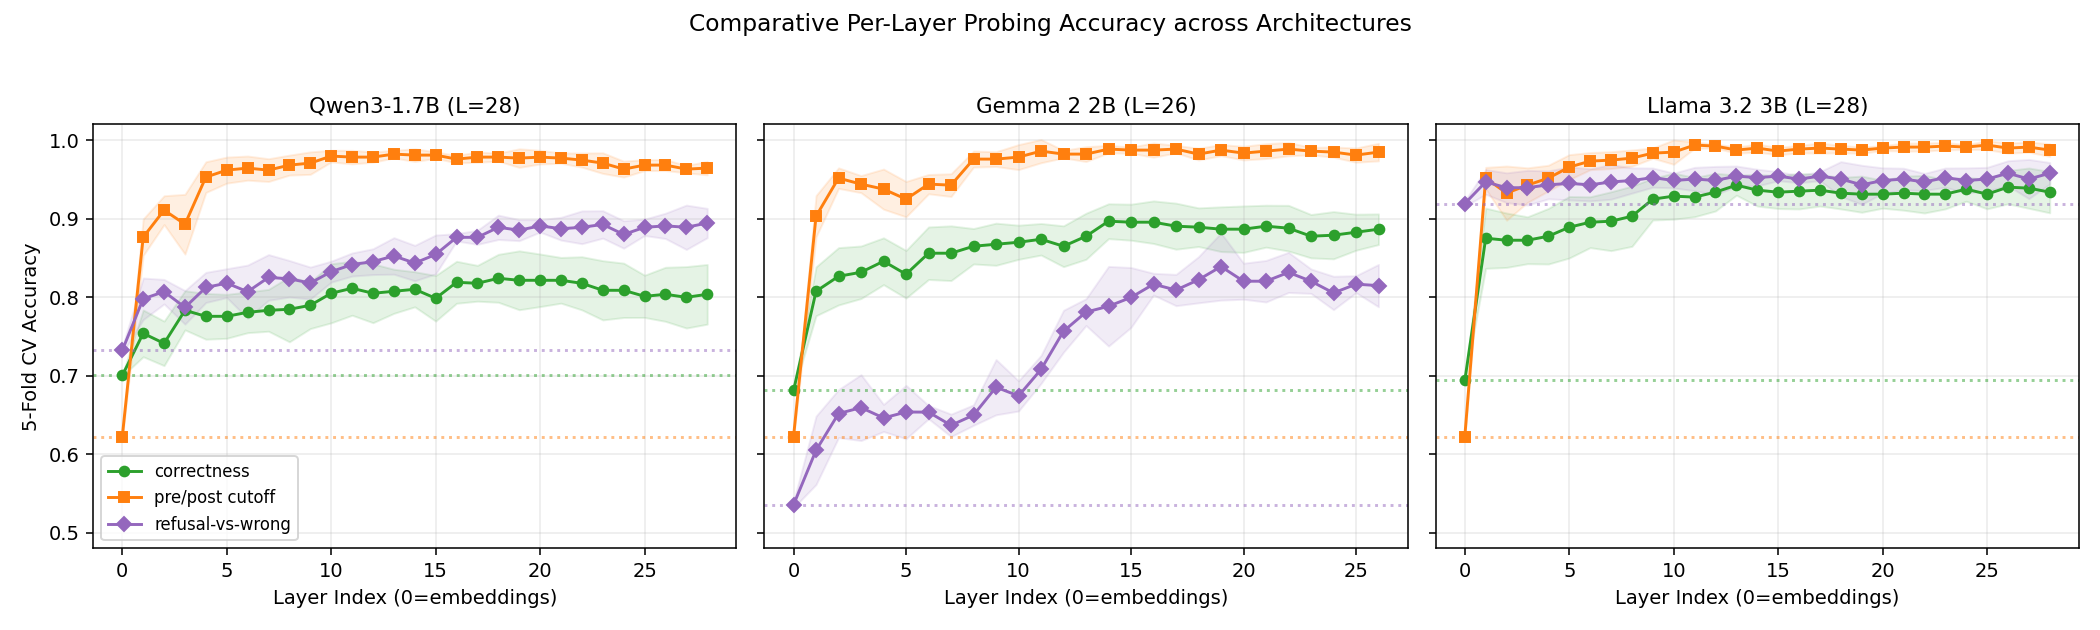
\includegraphics[keepaspectratio,alt={Comparative probing accuracy curves
  across Qwen3-1.7B, Gemma 2 2B, and Llama 3.2 3B.}]{figures/comparative_probes.png}}
\caption{Comparative probing accuracy curves across Qwen3-1.7B, Gemma 2
2B, and Llama 3.2 3B (Section 7.1).}\label{fig:comparative-probes}
\end{figure}

\subsubsection{D.6 Refusal-vs-wrong probe under class imbalance
(Section 5.5)}\label{refusal-vs-wrong-probe-under-class-imbalance}

Bare accuracy (\(0.894\)) is misleading for the
\texttt{refusal\_vs\_wrong} target because refusals are
\(147/549 = 26.8\%\) of the wrong+refusal subset: a constant predictor
of \texttt{wrong} already scores \(0.732\). At the peak layer (28) the
class-imbalance-aware metrics are: confusion matrix
\([[\mathrm{TN}, \mathrm{FP}], [\mathrm{FN}, \mathrm{TP}]] =
[[369, 33], [25, 122]]\), balanced accuracy \(0.874\), recall on
refusals \(122/147 = 0.830\), recall on wrong \(369/402 = 0.918\), ROC
AUC \(0.944\). The probe is not defaulting to ``wrong'': it flags 122 of
147 refusals at a false positive rate of \(33/402 \approx 8.2\%\), and
the AUC shows it ranks refusals well above confabulations in score
order.

\subsubsection{D.7 SAE feature-ranking views and the wrong-pole
search (Section 6.3)}\label{d.7-the-wrong-pole-feature-search}

\begin{figure}
\centering
\pandocbounded{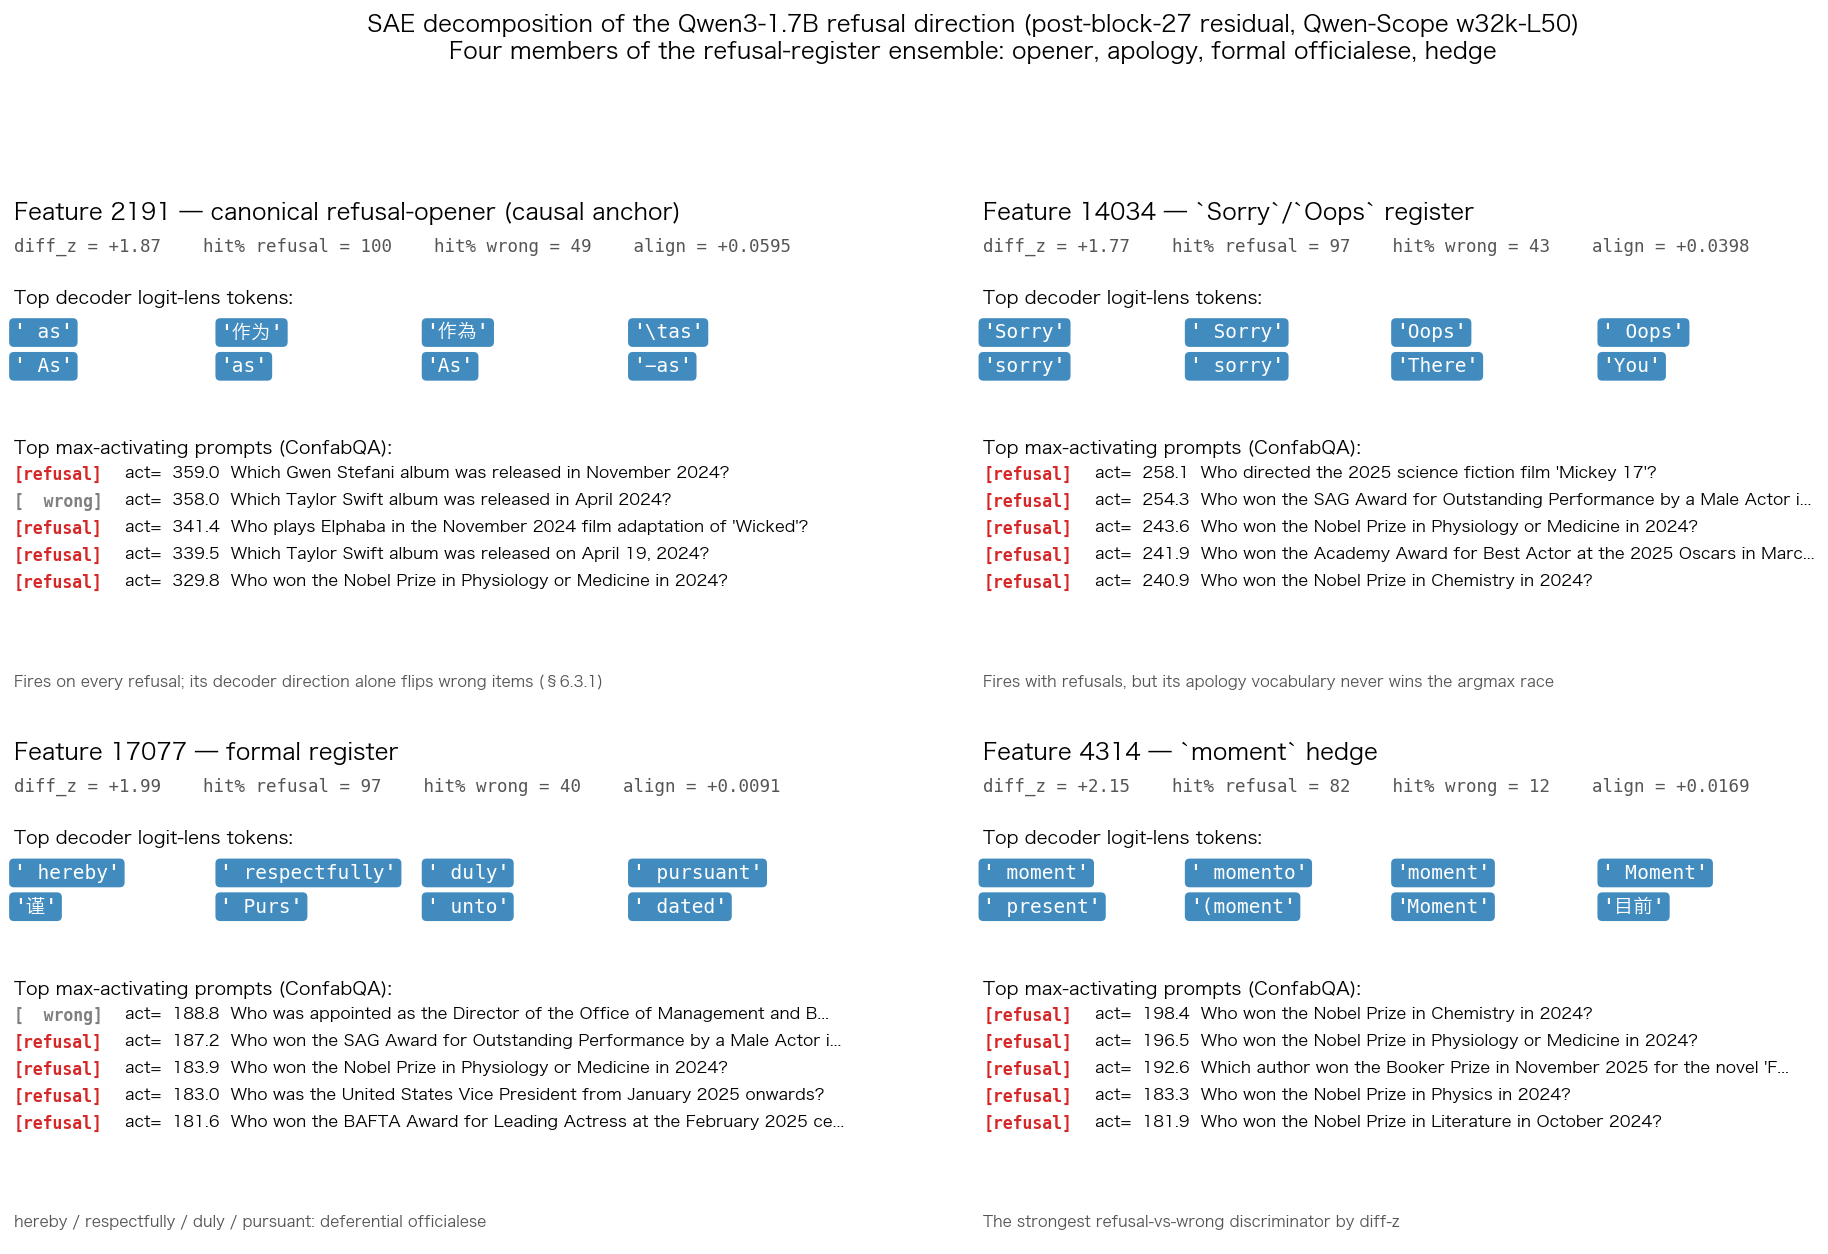
\includegraphics[keepaspectratio,alt={Four members of the refusal-register
  ensemble at the post-block-27 residual. Left column: the canonical refusal-opener (the
  Section 6.3.1 causal anchor) and the Sorry/Oops register. Right column: deferential
  officialese and the moment hedge. Hit rates and max-activating prompts are computed at
  the SAE's declared hook.},width=0.8\linewidth]{figures/sae_features_card.png}}
\caption{Four members of the refusal-register ensemble at the
post-block-27 residual. Left column: the canonical refusal-opener (the
Section 6.3.1 causal anchor) and the
\protect\texttt{Sorry}/\protect\texttt{Oops} register. Right column:
deferential officialese and the \protect\texttt{moment} hedge. Hit rates
and max-activating prompts are computed at the SAE's declared
hook.}\label{fig:sae-features}
\end{figure}

The three Section 6.3 views, for each of the \(32{,}768\) features:
\textbf{(A) direct encoding}, the features the encoder allocates to the
direction placed at typical state magnitude
(\(\mathrm{SAE.encode}(\overline{\|h\|}\, \hat{w}_{\rm refusal})\);
the encoder is scale-sensitive); \textbf{(B) decoder alignment},
\(W_{\rm dec} \cdot w_{\rm refusal}\) per feature, independent of the
encoder nonlinearity; and \textbf{(C) empirical activation
differential}, the standardized gap between mean activation on refusal
items and wrong items, independent of the recovered direction.
Convergent features are the most interpretable. Ensemble-member detail
behind the Section 6.3 roster: the \texttt{moment} hedge 4314
(diff-\(z\) \(+2.15\), the strongest discriminator) fires on \(82\%\) of
refusals vs \(12\%\) of wrongs, and its max-activating prompts are
post-cutoff prize questions the model refuses; officialese 17077
(\texttt{hereby}, \texttt{respectfully}, \texttt{duly},
\texttt{pursuant}) fires on \(97\%\) of refusals vs \(40\%\) of
wrongs; the
polite-modality feature 14361 reads \texttt{may}, \texttt{Please},
\texttt{Hopefully}; the first-person feature 8875 reads \texttt{I},
\texttt{我}; 14034 is a register feature whose output vocabulary always
loses the argmax race to ``As''; and 2191's max-activating prompts are
the recent-date items the model declines (Nov 2024 Gwen Stefani album,
the \emph{Wicked} adaptation, Taylor Swift album dates).

The strongest wrong-vs-correct feature in the Section 6.3 mirror search
is a \emph{topic} cue, not a commitment marker: an award-vocabulary
detector (lens \texttt{winning}, \texttt{荣获}, \texttt{获得}) firing
on \(22\%\) of wrong items vs.~\(1\%\) of correct and \(0\%\) of
refusals, whose max-activating prompts are the obscure Best Picture
years of the model's weakest cell; it tops the disconfounded within-pre
ranking too (diff-\(z\) \(+1.34\)). The runners-up are of the same
species (a Nobel-Prize topic feature, an ``In {[}date{]}'' phrasing
feature, a question-form feature), and against refusals the top
wrong-side features are attempt and formatting features that fire on
correct and wrong items alike. What the search rules out is a
concentrated confabulation marker in this dictionary, the mirror image
of 2191.

% ----- E. Bootstrap protocol and attribution details -----
\subsection{E. Bootstrap protocol and attribution
details}\label{e.-bootstrap-protocol-and-attribution-details}

Supporting protocol and accounting detail for Sections 8.1--8.3.

Table \ref{tbl:bootstrap} is the Section 8.1 bootstrap table in full;
Figure \ref{fig:bootstrap-forest} is its forest plot.

\begin{table}[!htbp]
\small
\centering
\caption{Bootstrap 95\% CIs on \(h_{adds}\) across the 14 (dataset,
model, target) cells; forest plot in Appendix E (Figure
\ref{fig:bootstrap-forest}).\label{tbl:bootstrap}}
\begin{tabular}{@{}
  >{\raggedright\arraybackslash}p{(\linewidth - 12\tabcolsep) * \real{0.2588}}
  >{\raggedright\arraybackslash}p{(\linewidth - 12\tabcolsep) * \real{0.1765}}
  >{\raggedright\arraybackslash}p{(\linewidth - 12\tabcolsep) * \real{0.1765}}
  >{\raggedleft\arraybackslash}p{(\linewidth - 12\tabcolsep) * \real{0.0588}}
  >{\raggedleft\arraybackslash}p{(\linewidth - 12\tabcolsep) * \real{0.0706}}
  >{\raggedright\arraybackslash}p{(\linewidth - 12\tabcolsep) * \real{0.1882}}
  >{\centering\arraybackslash}p{(\linewidth - 12\tabcolsep) * \real{0.0706}}@{}}
\toprule
\begin{minipage}[b]{\linewidth}\raggedright
dataset
\end{minipage} & \begin{minipage}[b]{\linewidth}\raggedright
model
\end{minipage} & \begin{minipage}[b]{\linewidth}\raggedright
target
\end{minipage} & \begin{minipage}[b]{\linewidth}\raggedleft
\(n\)/class
\end{minipage} & \begin{minipage}[b]{\linewidth}\raggedleft
\(\bar h_{adds}\)
\end{minipage} & \begin{minipage}[b]{\linewidth}\raggedright
95\% CI
\end{minipage} & \begin{minipage}[b]{\linewidth}\centering
excl 0?
\end{minipage} \\\midrule
ConfabQA & Qwen3-1.7B & correct (all) & 235 & \(+4.30\) &
\([+1.70, +7.45]\) & \textbf{yes} \\
ConfabQA & Qwen3-1.7B & within\_pre & 140 & \(+1.25\) &
\([-1.07, +3.57]\) & no \\
ConfabQA & Qwen3-1.7B & within\_obscure & 51 & \(+0.95\) &
\([-2.05, +6.90]\) & no \\
ConfabQA & Gemma 2 2B & correct (all) & 250 & \(+4.98\) &
\([+2.40, +7.20]\) & \textbf{yes} \\
ConfabQA & Gemma 2 2B & within\_pre & 90 & \(+2.54\) &
\([-0.56, +5.00]\) & no \\
ConfabQA & Gemma 2 2B & within\_obscure & 55 & \(+2.76\) &
\([-0.91, +6.36]\) & no \\
ConfabQA & Llama 3.2 3B & correct (all) & 240 & \(+0.94\) &
\([+0.21, +1.88]\) & \textbf{yes} \\
ConfabQA & Llama 3.2 3B & within\_pre & 57 & \(+11.43\) &
\([+5.18, +19.45]\) & \textbf{yes} \\
ConfabQA & Llama 3.2 3B & within\_obscure & 38 & \(+12.26\) &
\([+2.67, +23.67]\) & \textbf{yes} \\
PopQA & Qwen3-1.7B & correct (full) & 354 & \(+4.35\) &
\([+2.11, +6.50]\) & \textbf{yes} \\
PopQA & \textbf{Qwen3-4B} (within-family scaling) & correct (full) & 129
& \(+5.77\) & \([+2.34, +11.61]\) & \textbf{yes} \\
TriviaQA & Qwen3-1.7B & correct (full) & 400 & \(+9.57\) &
\([+5.13, +13.75]\) & \textbf{yes} \\
\textbf{PopQA} & \textbf{Llama 3.2 3B} & correct (full) & \(131\) &
\(\mathbf{+24.94}\) & \(\mathbf{[+20.57, +29.03]}\) & \textbf{yes} \\
\textbf{TriviaQA} & \textbf{Llama 3.2 3B} & correct (full) & \(356\) &
\(\mathbf{+21.25}\) & \(\mathbf{[+19.52, +22.89]}\) & \textbf{yes} \\
\bottomrule
\end{tabular}
\end{table}


\begin{figure}
\centering
\pandocbounded{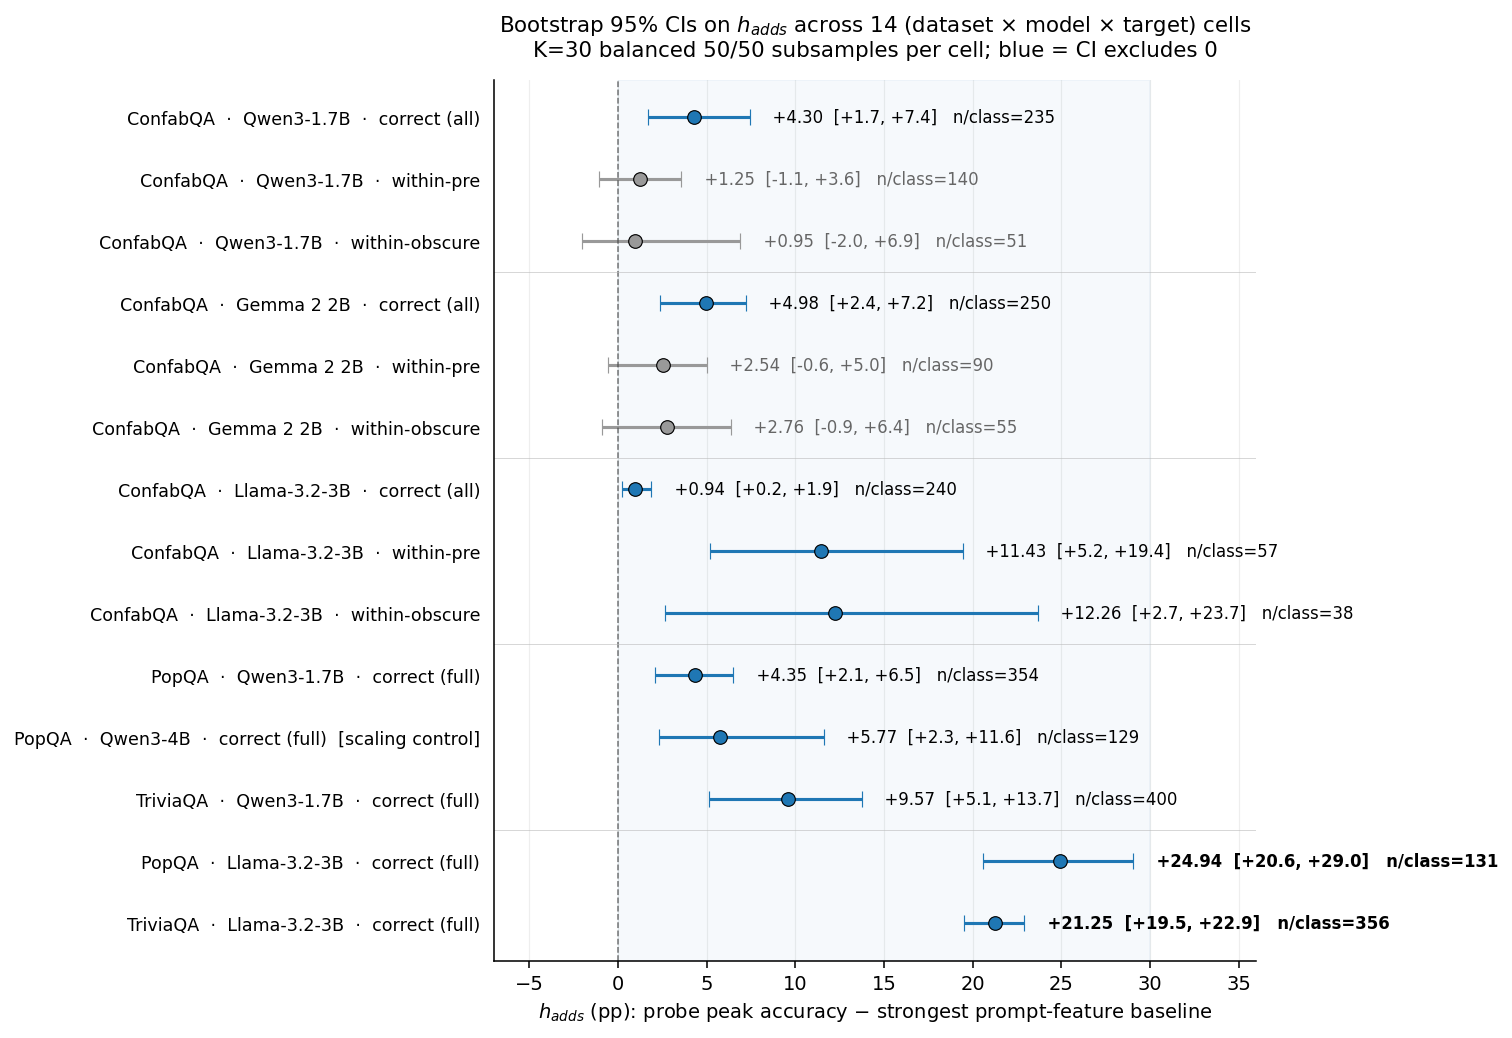
\includegraphics[keepaspectratio,alt={Bootstrap 95\% CIs on h\_\{adds\}
  across 14 (dataset, model, target) cells. K=30 balanced 50/50 subsamples per cell; blue
  = CI excludes 0. The bottom two rows are the headline positive finding: Llama 3.2 3B on
  PopQA / TriviaQA recovers +21--+25 pp over the strongest prompt-feature baseline, where
  Qwen3-1.7B and Qwen3-4B on the same data recover +4--+10 pp. The Qwen3-4B row labeled
  ``scaling control'' rules out parameter count as the dominant driver of the cross-model
  gap.}]{figures/bootstrap_forest.png}}
\caption{Forest plot of the Table \ref{tbl:bootstrap} bootstrap 95\% CIs
on \(h_{adds}\) across \(14\) \protect\texttt{(dataset,\ model,\ target)}
cells. \(K=30\) balanced 50/50 subsamples per cell; blue = CI excludes
0. The bottom two rows are the headline positive finding: Llama 3.2 3B
on PopQA / TriviaQA recovers \(+21\)--\(+25\) pp over the strongest
prompt-feature baseline, where Qwen3-1.7B and Qwen3-4B on the
\emph{same} data recover \(+4\)--\(+10\) pp. The Qwen3-4B ``scaling
control'' row rules out parameter count as the dominant driver of the
cross-model gap.}\label{fig:bootstrap-forest}
\end{figure}

\textbf{Bootstrap protocol detail (Sections 4, 8.1).} Per cell,
\(n_{\text{class}} = \min(|\rm pos|, |\rm neg|, 400)\); each subsample's
\(h_{\rm adds}\) is \(\text{probe peak} - \max(\text{baselines})\)
in\,\%, the reported \(\bar h_{\rm adds}\) is the mean across \(K\), and
the 95\% CI is the percentile interval
\([h_{(0.025K)}, h_{(0.975K)}]\). \(K=30\) is set by
compute (each replicate refits the full \(29\)-layer \(\times\)
\(5\)-fold pipeline), and percentile CIs at \(K=30\) are correspondingly
coarse. The protocol is ``resampling-of-balanced-subsamples'' rather
than a true item-level bootstrap; the latter would require
\(K \cdot L \cdot F \approx 4{,}350\) refits per cell, too slow on
M1-class hardware (see the evaluation-methodology limitation in Section
10).

\textbf{Permutation-null and item-level-bootstrap calibrations (Section
8.1).} Two protocol checks calibrate the Table \ref{tbl:bootstrap} CIs
(artifact \texttt{small\_cell\_stats}; fixed layer, TF-IDF baseline, so
absolute values are not comparable to the table). First, a
label-permutation null of the peak-over-all-layers margin measures the
layer-selection bias directly: null mean \(+0.6\) pp, 95th percentile
\(+1.3\) pp on both models, so margins in the \(\approx 1\) pp range
(e.g.\ Llama ConfabQA correct, \(+0.94\)) should not be read as
evidence, while the all-items margins sit far above the null
(\(p < 0.01\)). Second, an item-level bootstrap (\(B = 400\)) keeps the
Llama all-items margin positive (CI excluding zero) but leaves
\emph{both} Llama within-stratum cells consistent with zero (within-pre
\([-2.0, +8.5]\), within-obscure \([-3.3, +11.8]\)): the subsample
protocol's positive CIs for those two cells understate item-sampling
uncertainty and should be read as point estimates.

\textbf{External-dataset sampling (Section 4).} Both external datasets
run through the \texttt{02\_evaluate.py} generation pipeline. PopQA:
\(14\)k Wikidata
triples templated into natural-language questions; sampled \(n=800\)
stratified by \texttt{o\_pop} (object popularity, \(5\) quintile bins of
\(160\) items each), reshuffled at \texttt{seed} \(\in \{0, 1, 2\}\).
TriviaQA: \texttt{mandarjoshi/trivia\_qa\ unfiltered.nocontext}
validation split; sampled \(n=800\) uniformly, reshuffled at
\texttt{seed} \(\in \{0, 1, 2\}\). Generation settings match ConfabQA:
greedy decoding, \texttt{enable\_thinking=False}, last-prompt-token
hidden-state capture at every layer.

\textbf{Transfer-grid mechanics (Section 8.3).} The fitted pipeline is
transferred with its scaler and PCA held fixed at the source-dataset
statistics; only evaluation touches the target dataset. The sweep uses a
fixed four-layer grid per model (Qwen \(\{14,18,22,28\}\), Gemma
\(\{6,13,20,26\}\), Llama \(\{7,14,21,28\}\)); the Section 8.3 headline
rows report the grid layer closest to each model's Table
\ref{tbl:crossmodel} peak (Qwen \(18\), Gemma \(13\), Llama \(14\)), and
the full grids are in the released matrices. A prompt-feature-only
baseline (TF-IDF on question text) is fit on the same splits as a
control: if the hidden-state probe transferred worse than the
prompt-feature classifier, the hidden state would have contributed
nothing portable beyond what the question text already encoded.

\textbf{Transfer results in full (Section 8.3).} Table
\ref{tbl:transfer} is the headline retention summary; the per-model
readings follow.

\begin{table}[!htbp]
\small
\centering
\caption{Cross-dataset transfer at each model's peak-within layer:
margin retention without refit.\label{tbl:transfer}}
\begin{tabular}{@{}
  >{\raggedright\arraybackslash}p{(\linewidth - 10\tabcolsep) * \real{0.2250}}
  >{\raggedleft\arraybackslash}p{(\linewidth - 10\tabcolsep) * \real{0.1000}}
  >{\raggedleft\arraybackslash}p{(\linewidth - 10\tabcolsep) * \real{0.1625}}
  >{\raggedleft\arraybackslash}p{(\linewidth - 10\tabcolsep) * \real{0.1750}}
  >{\raggedleft\arraybackslash}p{(\linewidth - 10\tabcolsep) * \real{0.1125}}
  >{\raggedleft\arraybackslash}p{(\linewidth - 10\tabcolsep) * \real{0.2250}}@{}}
\toprule
\begin{minipage}[b]{\linewidth}\raggedright
Model
\end{minipage} & \begin{minipage}[b]{\linewidth}\raggedleft
Peak layer
\end{minipage} & \begin{minipage}[b]{\linewidth}\raggedleft
Avg within margin
\end{minipage} & \begin{minipage}[b]{\linewidth}\raggedleft
Avg transfer margin
\end{minipage} & \begin{minipage}[b]{\linewidth}\raggedleft
Retention
\end{minipage} & \begin{minipage}[b]{\linewidth}\raggedleft
Transfers \(>\) majority
\end{minipage} \\\midrule
Llama 3.2 3B & 14 & \(+18.9\) pp & \(+15.2\) pp & \(81\%\) & \(5/6\) \\
Gemma 2 2B & 13 & \(+13.1\) pp & \(-7.0\) pp & \(-54\%\) & \(4/6\) \\
Qwen3-1.7B & 18 & \(+8.7\) pp & \(-1.2\) pp & \(-14\%\) & \(3/6\) \\
\bottomrule
\end{tabular}
\end{table}

\textbf{Llama: content-invariant.} Five of six off-diagonal transfers
beat the test-dataset majority, with an average winning margin of
\(+19.8\) pp, comparable to the within-dataset \(+18.9\) pp. The single
failure is ConfabQA \(\to\) PopQA (majority \(87.3\%\), transfer
\(79.8\%\)). Two transfer cells (PopQA \(\to\) ConfabQA at \(94.0\%\),
TriviaQA \(\to\) ConfabQA at \(93.8\%\)) actually exceed the
within-ConfabQA CV accuracy of \(93.5\%\), suggesting less overfit when
trained on more diverse data than ConfabQA alone provides.

\textbf{Gemma: strong within, collapsed transfer.} Gemma has the
\emph{largest} average within-dataset margin of the three at this layer
but the worst transfer. Two cells collapse catastrophically, both with
PopQA as target: ConfabQA \(\to\) PopQA at \(38.3\%\) (vs majority
\(80.2\%\), a \(-42\) pp gap) and TriviaQA \(\to\) PopQA at \(46.8\%\)
(\(-33.5\) pp). Four cells do beat majority (transfers to ConfabQA and
TriviaQA), average winning margin \(+8.3\) pp, well below Llama's
\(+19.8\); the net signed average is \(-7.0\) pp, dominated by the PopQA
collapses.

\textbf{Qwen: weak within, weak transfer.} Qwen3-1.7B's within-dataset
margins are the smallest to begin with (\(+8.7\) pp average); three of
six transfers beat majority, all by small amounts (\(+1.7\) to
\(+7.7\) pp). Its signed transfer average (\(-1.2\) pp) is closer to zero
than Gemma's not because Qwen transfers better but because an almost
flat probe stays almost flat under transfer (retention \(-14\%\)).


\textbf{Refusal census (Section 8.2) and Qwen3-4B raw accuracies
(Section 8.1).} Pool-level refusal rates behind
the Section 8.2 anchor: Llama PopQA \(62.9\%\) vs.~Qwen \(1.7\%\)
(\(39/2264\) refusals in the pooled three-seed Qwen sample); Llama
TriviaQA \(31.5\%\) vs.~Qwen \(1.2\%\) (\(28/2242\)). The four
attribution cells are Qwen \(\times\) \{PopQA, TriviaQA\} and Llama
\(\times\) \{PopQA, TriviaQA\}. Qwen3-4B's PopQA judge breakdown
(\(14.8\%\) correct / \(1.6\%\) refusal / \(83.6\%\) wrong) is
essentially Qwen3-1.7B's, and the family's \(\approx 2\%\) refusal rate
versus Llama's \(63\%\) on the same items is the conspicuous
family-level difference.

\textbf{Refusal-channel attribution: full results (Section 8.2).}
Table \ref{tbl:refchannel} gives both tests in full.

\begin{table}[!htbp]
\small
\centering
\caption{Refusal-channel attribution: Test A (drop refusals) and Test B
(probe refusal directly).\label{tbl:refchannel}}
\begin{tabular}{@{}
  >{\raggedright\arraybackslash}p{(\linewidth - 14\tabcolsep) * \real{0.2073}}
  >{\raggedright\arraybackslash}p{(\linewidth - 14\tabcolsep) * \real{0.1098}}
  >{\raggedright\arraybackslash}p{(\linewidth - 14\tabcolsep) * \real{0.1707}}
  >{\raggedleft\arraybackslash}p{(\linewidth - 14\tabcolsep) * \real{0.0610}}
  >{\raggedleft\arraybackslash}p{(\linewidth - 14\tabcolsep) * \real{0.0854}}
  >{\raggedleft\arraybackslash}p{(\linewidth - 14\tabcolsep) * \real{0.0854}}
  >{\raggedleft\arraybackslash}p{(\linewidth - 14\tabcolsep) * \real{0.0854}}
  >{\raggedright\arraybackslash}p{(\linewidth - 14\tabcolsep) * \real{0.1951}}@{}}
\toprule
\begin{minipage}[b]{\linewidth}\raggedright
Test
\end{minipage} & \begin{minipage}[b]{\linewidth}\raggedright
dataset
\end{minipage} & \begin{minipage}[b]{\linewidth}\raggedright
model
\end{minipage} & \begin{minipage}[b]{\linewidth}\raggedleft
\(n\)/class
\end{minipage} & \begin{minipage}[b]{\linewidth}\raggedleft
probe acc
\end{minipage} & \begin{minipage}[b]{\linewidth}\raggedleft
strongest baseline
\end{minipage} & \begin{minipage}[b]{\linewidth}\raggedleft
\(h_{adds}\)
\end{minipage} & \begin{minipage}[b]{\linewidth}\raggedright
95\% CI
\end{minipage} \\\midrule
A: drop refusals & PopQA & Qwen3-1.7B & 355 & 79.18\% & 75.87\% &
\(+3.31\) & \([+1.55, +6.48]\) \\
A: drop refusals & PopQA & Llama 3.2 3B & 102 & 82.37\% & 61.61\% &
\(\mathbf{+20.76}\) & \(\mathbf{[+14.67, +27.94]}\) \\
A: drop refusals & TriviaQA & Qwen3-1.7B & 400 & 69.40\% & 60.04\% &
\(+9.36\) & \([+6.50, +12.87]\) \\
A: drop refusals & TriviaQA & Llama 3.2 3B & 179 & 74.23\% & 56.52\% &
\(\mathbf{+17.71}\) & \(\mathbf{[+13.43, +21.78]}\) \\
B: probe refusal & PopQA & Qwen3-1.7B & \(39\) & 86.27\% & 76.04\% &
\(+10.24\) & \([\mathit{0.00}, +20.42]\) \\
B: probe refusal & PopQA & Llama 3.2 3B & 297 & 84.47\% & 66.03\% &
\(\mathbf{+18.44}\) & \(\mathbf{[+16.16, +21.72]}\) \\
B: probe refusal & TriviaQA & Qwen3-1.7B & \(28\) & 73.34\% & 57.37\% &
\(+15.97\) & \([-3.48, +32.27]\) \\
B: probe refusal & TriviaQA & Llama 3.2 3B & 252 & 90.23\% & 64.80\% &
\(\mathbf{+25.43}\) & \(\mathbf{[+22.81, +29.76]}\) \\
\bottomrule
\end{tabular}
\end{table}

(Italicized CI lower bound: 95\% CI includes 0 because the refusal count
is too small for the \(K=30\) percentile bootstrap to be well-resolved.)

\textbf{Reading Test A.} Comparing the drop-refusals rows to the
unfiltered Table \ref{tbl:bootstrap} rows: for Llama,
\(+24.94 \to +20.76\) on PopQA and \(+21.25 \to +17.71\) on TriviaQA,
i.e.~the refusal channel accounts for \(\approx 17\%\) of the headline
and the bulk (\(\approx 83\%\)) is real correct-vs-wrong discrimination
on attempted items. The refusal-channel hypothesis is \emph{partially}
right (about a sixth of the signal) but cannot account for the gap with
Qwen, which would require nearly all of it. The Qwen rows are
essentially unchanged (\(+4.35 \to +3.31\) PopQA, \(+9.57 \to +9.36\)
TriviaQA): Qwen refuses too rarely on these benchmarks for
refusal-readout to be a substantial confound either way. One caveat on
the ratio: its numerator is judge-labeled and its denominator
substring-labeled (Appendix E). A label-sensitivity rerun (single
pipeline, both regimes; artifact \texttt{small\_cell\_stats}) shows
the contrast is not a label artifact: under judge labels Llama's
TriviaQA margin grows (\(+17.5 \to +23.8\) in that pipeline) and the
Llama-vs-Qwen ordering is unchanged on both external datasets.

\textbf{Reading Test B.} Llama's refusal probe reaches \(84.5\%\)
(PopQA) and \(90.2\%\) (TriviaQA) absolute accuracy on a balanced 50/50
task, beating the strongest prompt baseline by \(+18.4\) and
\(+25.4\) pp, CIs excluding \(0\) by wide margins: the hidden state
encodes the abstention decision in a form the question text does not
predict. Qwen's analogous margins (\(+10.2\) pp PopQA, \(+16.0\) pp
TriviaQA) are positive but the refusal counts (\(39\) and \(28\)) leave
the CIs straddling \(0\); this test needs either a larger Qwen
evaluation or a benchmark on which Qwen3 refuses more (Qwen refuses
\(37.4\%\) on ConfabQA's post-cutoff stratum).


\textbf{Label provenance (Section 8.1).} For the ConfabQA cells the
\texttt{correct} field is the three-way judge's label (Section 5); for
the external-dataset cells it is the generation-time substring match
against gold and alternatives (the judge pass post-dates these bootstrap
runs). Section 8.2's attribution tests use the judge labels instead,
which is why their per-class counts differ from Table
\ref{tbl:bootstrap}'s (e.g.~Llama PopQA: \(131\) substring-correct
vs.~\(102\) judge-correct).

\textbf{Accuracy and baseline accounting for the Section 8.1 contrast.}
PopQA substring-correct rates are nearly identical (\(16.4\%\) Llama
vs.~\(15.6\%\) Qwen); on TriviaQA Llama is more accurate (\(44.5\%\)
vs.~\(27.4\%\)), but 50/50 balancing removes any base-rate advantage.
Llama's strongest PopQA dropped-refusals prompt baseline is \(61.6\%\)
vs.~Qwen's \(75.9\%\), so a lower baseline floor does not explain the
gap either.

% ----- F. Extended discussion -----
\subsection{F. Extended discussion}\label{f.-extended-discussion}

The Section 9 readings in full.

\textbf{The robust positive result.} The refusal direction's logit lens
recovers the literal refusal-opening vocabulary in each model (Qwen3:
\texttt{as}, \texttt{As}, \texttt{作为}; Gemma: \texttt{Regret},
\texttt{Formal}, \texttt{Alas}; Llama: \texttt{I}, \texttt{Given},
\texttt{As}), the one-shot intervention drives the first-token opener
rate to \(100\%\) on Qwen3 and Gemma (Sections 6.2, 7.2), and the
Section 8.2 refusal probe extends the finding to PopQA and TriviaQA at
Llama scale; the claim ``refusal is a clean, late-network,
linearly-decodable, causally-load-bearing direction in these three small
LMs'' survives the bootstrap and the external benchmarks, and is no
supervised artifact, being visible in unsupervised PCA (Figure
\ref{fig:atlas}b, Figure \ref{fig:embeddings}). The Qwen3-1.7B
correctness direction fails all three corresponding tests: little margin
over the difficulty oracle (Table \ref{tbl:hadds}), no token-space
signature, no sign-directional causal effect (Section 6.2).

\textbf{Why two atlases on Llama, one on Qwen.} A plausible mechanism:
Llama's heavier calibrated-abstention training requires a
distinguishable internal ``I should hedge'' state (the Test-B gap) and a
richer correctness representation as its \emph{prerequisite} (what Test
A recovers); Qwen3-1.7B, which prefers to attempt-and-confabulate, never
had pressure to develop either. The Qwen3-4B scaling control supports
this: same family, same near-zero PopQA refusal rate, \(h_{adds}\)
essentially at Qwen3-1.7B's level and far below Llama's. The mechanism
is family / post-training recipe, not scale; a fully clean ablation
would still need a recipe swap holding family fixed, which is future
work.

\textbf{Implication for the probing literature.} Probing papers
reporting ``the hidden state predicts correctness at
\(\sim 80\)--\(90\%\)'' should be re-evaluated against a prompt-feature
baseline (removing the cutoff variable is necessary but not sufficient),
and the result is sharply model-dependent: a single-model study could
report either ``substantial factual self-knowledge'' (Llama) or
``nothing over prompt features'' (Qwen ConfabQA within-obscure) on
identical data and code, consistent with \citeauthor{orgad2024show}'s (\citeyear{orgad2024show}) finding
that truthfulness encoding is multifaceted rather than universal.
Headline small-LM claims should be checked on at least two architectures
with different post-training recipes, with bootstrap CIs on balanced
subsamples rather than single-seed point estimates. Finally, the refusal
direction is a structure of the continuous representation space that
becomes text one token later; a natural extension is to measure
calibration directly in that space (signed distances to the refusal and
correctness hyperplanes as continuous confidence scores).

